\chapter{Linear Algebra}


\section{Fields}

This section focuses on key properties of the real and complex numbers that make them useful for linear algebra.
Consider a set $F$ of objects and two operations on the elements of $F$, addition and multiplication.
For every pair of elements $s, t \in F$ then their sum $(s + t) \in F$.
For every pair of elements $s, t \in F$ then their product $st \in F$.
Suppose that these two operations satisfy
\begin{enumerate}
\item addition is commutative: $s + t = t + s \; \forall s, t \in F$
\item addition is associative: $r + (s + t) = (r + s) + t \; \forall r, s, t \in F$
\item to each $s \in F$ there exists a unique element $(-s) \in F$ such that $s + (-s) = 0$
\item multiplication is commutative: $st = ts \; \forall s,t \in F$
\item multiplication is associative: $r(st) = (rs)t \; \forall r, s, t \in F$
\item there is a unique non-zero element $1 \in F$ such that $s1 = s \; \forall s \in F$
\item to each $s \in F - 0$ there exists a unique element $s^{-1} \in F$ such that $s s^{-1} = 1$
\item multiplication distributes over addition: $r (s + t) = rs + rt \; \forall r, s, t \in F$.
\end{enumerate}
Then, the set $F$ together with these two operations is a \textbf{field}.
\index{field}

\begin{example}
The real numbers with the usual operations of addition and multiplication form a field.
The complex numbers with these two operations also form a field.
\end{example}

\begin{example}
The set of integers with addition and multiplication is not a field.
\end{example}

\begin{problem} \label{problem:RationalNumbers}
Is the set of rational numbers a subfield of the real numbers?
\end{problem}

\begin{example}
Is the set of all real numbers of the form $s + t \sqrt{2}$, where $s$ and $t$ are rational, a subfield of the complex numbers?

The set $F = \left\{ s + t \sqrt{2} : s, t \in \RationalNumbers \right\}$ together with the standard addition and multiplication is a field.
Let $s, t, u, v \in \RationalNumbers$,
\begin{gather*}
s + t \sqrt{2} + u + v \sqrt{2} = (s+u) + (t+v) \sqrt{2} \in F \\
\left( s + t \sqrt{2} \right) \left( u + v \sqrt{2} \right) = (su + 2 tv) + (sv + tu) \sqrt{2} \in F \\
\left( s + t \sqrt{2} \right)^{-1} = \frac{ s - t \sqrt{2} }{ s^2 + 2 t^2 }
= \frac{ s }{ s^2 + 2 t^2 } - \frac{ t }{ s^2 + 2 t^2 } \sqrt{2} \in F
\end{gather*}
Again, the remaining properties are straightforward to prove.
The field $s + t \sqrt{2}$, where $s$ and $t$ are rational, is a subfield of the complex numbers.
\end{example}


\section{Matrices}

Let $F$ be a field and consider the problem of finding $n$ scalars $x_1, \ldots, x_n$ which satisfy the conditions
\begin{equation} \label{equation:SystemOfEquations}
\begin{array}{ccccccccc}
a_{11} x_1 & + & a_{12} x_2 & + & \cdots & + & a_{1n} x_n & = & y_1 \\
a_{21} x_1 & + & a_{22} x_2 & + & \cdots & + & a_{2n} x_n & = & y_2 \\
\vdots & & \vdots  & & & & \vdots & & \vdots \\
a_{m1} x_1 & + & a_{m2} x_2 & + & \cdots & + & a_{mn} x_n & = & y_m
\end{array}
\end{equation}
where $y_1,\ldots,y_n \in F$ and $a_{ij} \in F$ for $1 \leq i \leq m$ and $1 \leq j \leq n$.
These conditions form a \emph{system of $m$ linear equations in $n$ unknowns}.
A shorthand notation for~\eqref{equation:SystemOfEquations} is the matrix equation
\begin{equation*}
A \vecnot{x} = \vecnot{y},
\end{equation*}
where
$\vecnot{x} = (x_1, \ldots, x_n)^T$, 
$\vecnot{y} = (y_1, \ldots, y_m)^T$, and
$A$ is the matrix given by
\begin{equation*}
A = \begin{bmatrix}
a_{11} & a_{12} & \cdots & a_{1n} \\
a_{21} & a_{22} & \cdots & a_{2n} \\
\vdots & \vdots & \ddots & \vdots \\
a_{m1} & a_{m2} & \cdots & a_{mn}
\end{bmatrix}.
\end{equation*}
We also use $[A]_{i,j}$ to denote the entry of $A$ in the $i$-th row and $j$-th column (i.e., $a_{ij}$) and $[\vecnot{x}_i ]$ to denote the $i$-th entry in $\vecnot{x}$ (i.e., $x_i$).
%The vectors $\vecnot{x}$ and %$\vecnot{y}$ denoted by
%\begin{align*}
%\vecnot{x} &= (x_1, \ldots, x_n)^T \\
%\vecnot{y} &= (y_1, \ldots, y_m)^T .
%\end{align*}

\begin{definition}
Let $A$ be an $m \times n$ matrix over $F$ and let $B$ be an $n \times p$ matrix over $F$.
The \defn{matrix}{matrix product} $AB$ is the $m \times p$ matrix $C$ whose $i,j$ entry is
\begin{equation} \label{eq:def_matrix_product}
c_{ij} = \sum_{r = 1}^n a_{ir} b_{rj}.
\end{equation}
\end{definition}

\begin{remark}
Consider~\eqref{eq:def_matrix_product} when $j$ is fixed and $i$ is eliminated by grouping the elements of $C$ and $A$ into column vectors $\vecnot{c}_1,\ldots,\vecnot{c}_{p}$ and $\vecnot{a}_1,\ldots,\vecnot{a}_n$. For this case, \eqref{eq:def_matrix_product}~shows that the $j$-th column of $C$ is a linear combination of the columns of $A$,
\[ \vecnot{c}_{j} = \sum_{r = 1}^n \vecnot{a}_r b_{rj}, \]
%with coefficients $b_{1,j},b_{2,j},\ldots,b_{m,j}$.
Similarly, one can fix $i$ and eliminate the index $j$ by grouping the elements of $C$ and $B$ into row vectors  $\vecnot{c}_1,\ldots,\vecnot{c}_{m}$ and $\vecnot{b}_1,\ldots,\vecnot{b}_n$.
Then, \eqref{eq:def_matrix_product}~shows that the $i$-th row of $C$ is a linear combination of the rows of $B$,
\[ \vecnot{c}_{i} = \sum_{r = 1}^n a_{ir} \vecnot{b}_r. \]
% with coefficients $b_{i,1},b_{i,2},\ldots,b_{i,n}$.
\end{remark}

\begin{definition}
Consider an $m \times n$ matrix $A$ with elements $a_{ij} \in F$.
The \defn{matrix}{transpose} of $A$ is the $n \times m$ matrix $B = A^T$ with elements defined by $b_{ij} = a_{ji}$.
\end{definition}

\begin{definition}
Consider a complex $m \times n$ matrix $A$ with elements $a_{ij} \in \mathbb{C}$.
Its \defn{matrix}{Hermitian transpose} $B = A^H$ is the $n \times m$ matrix with elements defined $b_{ij} = \overline{a_{ji}}$, where $\overline{a}$ denotes the complex conjugate of $a$.
\end{definition}

\begin{problem}
For matrices $A \in \mathbb{C}^{m\times p}$ and $B \in \mathbb{C}^{p \times n}$, show $(AB)^H = B^H A^H$.
\end{problem}

\begin{definition}
An $m\times n$ matrix $A$ over $F$ is in \defn{matrix}{row echelon form} if
\begin{enumerate}
\item all rows containing only zeros, if they exist, are the bottom of the matrix, and
\item For non-zero rows, the leading coefficient (i.e., the first non-zero element from the left) is strictly to the right of the leading coefficient of the row above it.
\end{enumerate}
These two conditions imply that entries below the leading coefficient in a column are zero.
A matrix is \textbf{column echelon form} if its transpose is in row echelon form.
\end{definition}

\begin{definition}
An $m\times n$ matrix $A$ over $F$ is in \defn{matrix}{reduced row echelon form} if it is in row echelon form and
\begin{enumerate}
\item every leading coefficient is 1, and
\item every leading coefficient is the only non-zero element in its column.
\end{enumerate}
\end{definition}

\begin{definition}
Let $A$ be an $n \times n$ matrix over $F$.
An $n \times n$ matrix $B$ is called the \defn{matrix}{inverse} of $A$ if
\begin{equation*}
AB = BA = I.
\end{equation*}
In this case, $A$ is called \defn{matrix}{invertible} and its inverse is denoted by $A^{-1}$.
\end{definition}

\begin{problem}
For a matrix $A\in \mathbb{C}^{n\times n}$, show that $(A^H)^{-1} = (A^{-1})^H$ if $A^{-1}$ exists.
\end{problem}

\begin{definition}
An \defn{matrix}{elementary row operation} on an $m \times n$ matrix consists of
\begin{enumerate}
\item multiplying a row by a non-zero scalar,
\item swapping two rows, or
\item adding a non-zero scalar multiple of one row to another row.
\end{enumerate}
An \defn{matrix}{elementary column operation} is the same but applied to the columns.
\end{definition}

\begin{lemma}
For any $m\times n$ matrix $A$ over $F$, there is an invertible $m \times m$ matrix $P$ over $F$ such that $R=PA$ is in reduced row echelon form.
\end{lemma}
\begin{proof}[Sketch of Proof]
This follows from the fact that elementary row operations (i.e., Gaussian elimination) can be used to reduce any matrix to reduced row echelon form.
To construct the $P$ matrix, one applies Gaussian elimination to the augmented matrix $A' = [A \; I]$.
This results in an augmented matrix $R' = [R\; P]$ in reduced row echelon form.
It follows that $R$ is also in reduced row echelon form.
Since elementary row operations can be implemented by (invertible) matrix multiplies on the left side, one also finds that $R' = P A'$, $R = PA$, and $P$ is invertible.
\end{proof}

\begin{lemma}
\label{lemma:widematrix_has_nullvector}
Let $A$ be an $m \times n$ matrix over $F$ with $m<n$.
Then, there exists a length-$n$ column vector $\vecnot{x} \neq \vecnot{0}$ (over $F$) such that $A \vecnot{x} = \vecnot{0}$.
\end{lemma}
\begin{proof}
First, we use row reduction to compute the reduced row echelon form $R=PA$ of $A$, where $P$ is invertible.
Then, we observe that the columns of $R$ containing leading elements can be combined in a linear combination to cancel any other column of $R$.
This allows us to construct a vector $\vecnot{x}$ satisfying $R\vecnot{x}=\vecnot{0}$ and thus $A \vecnot{x} = P^{-1} R \vecnot{x} = \vecnot{0}$.
\end{proof}

\section{Vector Spaces}

\index{vector space}
\begin{definition} \label{definition:VectorSpace}
A \textbf{vector space} consists of the following,
\begin{enumerate}
\item a field $F$ of scalars
\item a set $V$ of objects, called vectors
\item an operation called vector addition, which associates with each pair of vectors $\vecnot{v}, \vecnot{w} \in V$ a vector $\vecnot{v} + \vecnot{w} \in V$ such that
\begin{enumerate}
\item addition is commutative: $\vecnot{v} + \vecnot{w} = \vecnot{w} + \vecnot{v}$
\item addition is associative: $\vecnot{u} + (\vecnot{v} + \vecnot{w}) = (\vecnot{u} + \vecnot{v}) + \vecnot{w}$
\item there is a unique vector $\vecnot{0} \in V$ such that $\vecnot{v} + \vecnot{0} = \vecnot{v}$, $\forall \vecnot{v} \in V$
\item to each $\vecnot{v} \in V$ there is a unique vector $- \vecnot{v} \in V$ such that $\vecnot{v} + (- \vecnot{v}) = \vecnot{0}$
\end{enumerate}
\item an operation called scalar multiplication, which associates with each $s \in F$ and $\vecnot{v} \in V$ a vector $s \vecnot{v} \in V$ such that
\begin{enumerate}
\item $1 \vecnot{v} = \vecnot{v}$, $\forall \vecnot{v} \in V$
\item $(s_1 s_2) \vecnot{v} = s_1 ( s_2 \vecnot{v} )$
\item $s ( \vecnot{v} + \vecnot{w} ) = s \vecnot{v} + s \vecnot{w}$
\item $(s_1 + s_2) \vecnot{v} = s_1 \vecnot{v} + s_2 \vecnot{v}$.
\end{enumerate}
\end{enumerate}
\end{definition}

\begin{example}
Let $F$ be a field, and let $V$ be the set of all $n$-tuples $\vecnot{v} = (v_1, \ldots, v_n)$ of scalar $v_i \in F$.
If $\vecnot{w} = (w_1, \ldots, w_n)$ with $w_i \in F$, the sum of $\vecnot{v}$ and $\vecnot{w}$ is defined by
\begin{equation*}
\vecnot{v} + \vecnot{w} = (v_1 + w_1, \ldots, v_n + w_n).
\end{equation*}
The product of a scalar $s \in F$ and vector $\vecnot{v}$ is defined by
\begin{equation*}
s \vecnot{v} = (s v_1, \ldots, s v_n).
\end{equation*}
The set of $n$-tuples, denoted by $F^n$, with the vector addition and scalar product defined above forms a vector space.
This is the standard vector space for $F^n$.
\end{example}

\begin{example}
Let $X$ be a non-empty set and let $Y$ be a vector space over $F$.
Consider the set $V$ of all functions from $X$ into $Y$.
The sum of two vectors $f,g \in V$ is the function from $X$ into $Y$ defined by
\begin{equation*}
(f + g)(x) = f(x) + g(x) \quad \forall x \in X,
\end{equation*}
where the RHS uses vector addition from $Y$.
The product of scalar $s \in F$ and the function $f \in V$ is the function $sf$ defined by
\begin{equation*}
(sf)(x) = s f(x) \; \forall x \in X,
\end{equation*}
where the RHS uses scalar multiplication from $Y$.
This is the standard vector space of functions from a set $X$ to a vector space $Y$.
\end{example}

\begin{definition}
A vector $\vecnot{w} \in V$ is said to be a \defn{vector space}{linear combination} of the vectors $\vecnot{v}_1, \ldots, \vecnot{v}_n \in V$ provided that there exist scalars $s_1, \ldots, s_n \in F$ such that
\begin{equation*}
\vecnot{w} = \sum_{i=1}^n s_i \vecnot{v}_i.
\end{equation*}
\end{definition}

\subsection{Subspaces}

\begin{definition}
Let $V$ be a vector space over $F$.
A \defn{vector space}{subspace} of $V$ is a subset $W \subset V$ which is itself a vector space over $F$.
\end{definition}

\begin{fact}
A non-empty subset $W \subset V$ is a subspace of $V$ if and only if for every pair $\vecnot{w}_1, \vecnot{w}_2 \in W$ and every scalar $s \in F$ the vector $s \vecnot{w}_1 + \vecnot{w}_2$ is again in $W$.
\end{fact}
If $V$ is a vector space then the intersection of any collection of subspaces of $V$ is a subspace of $V$.

\begin{example}
Let $A$ be an $m \times n$ matrix over $F$.
The set of all $n \times 1$ column vectors $V$ such that
\begin{equation*}
\vecnot{v} \in V \implies A \vecnot{v} = \vecnot{0}
\end{equation*}
is a subspace of $F^{n \times 1}$.
\end{example}

\begin{definition}
Let $U$ be a set (or list) of vectors in $V$.
The \defn{vector space}{span} of $U$, denoted $\Span(U)$, is defined to be the set of all finite linear combinations of vectors in $U$.
%The \defn{vector space}{subspace spanned} by $U$ is defined to be the intersection $W$ of all subspaces of $V$ which contain $U$.
\end{definition}

The subspace spanned by $U$ can be defined equivalently as the intersection of all subspaces of $V$ that contain $U$.
To see this, we note that the intersection of all subspaces containing $U$ is a subspace containing $U$ because the intersection of subspaces is also a subspace.
The intersection cannot be larger than $U$, however, because $U$ is a subspace containing $U$.

\begin{definition}
Let $V$ be a vector space and $U,W$ be subspaces.
If $U,W$ are disjoint (i.e., $U\cap W = \{ \vecnot{0} \}$), their \defn{vector space}{direct sum} $U \oplus W$ is defined by
\[ U \oplus W \triangleq \{\vecnot{u}+\vecnot{w} | \vecnot{u} \in U, \vecnot{w} \in W \}. \]
\end{definition}

An important property of a direct sum is that any vector $\vecnot{v} \in U \oplus W$ has a unique decomposition $\vecnot{v} = \vecnot{u} + \vecnot{w}$ where $\vecnot{u} \in U$ and $\vecnot{w} \in W$.
 
\subsection{Bases and Dimensions}
\label{section:BasesAndDimensions}

The dimension of a vector space is defined using the concept of a basis.

\begin{definition}
Let $V$ be a vector space over $F$.
A list of vectors $\vecnot{u}_1, \ldots, \vecnot{u}_n \in V $ is called \defn{vector space}{linearly dependent} if there are scalars $s_1, \ldots, s_n \in F$, not all of which are $0$, such that
\begin{equation*}
\sum_{i=1}^n s_i \vecnot{u}_i = 0.
\end{equation*}
A list that is not linearly dependent is called \defn{vector space}{linearly independent}.
Similarly, a subset $U \subset V$ is called linearly dependent if there is a finite list $\vecnot{u}_1, \ldots, \vecnot{u}_n \in U$ of distinct vectors that is linearly dependent.
Otherwise, it is called linearly independent.
\end{definition}

A few important consequences follow immediately from this definition.
Any subset of a linearly independent set is also linearly independent.
Any set which contains the $\vecnot{0}$ vector is linearly dependent.
A set $U \subset V$ is linearly independent if and only if each finite subset of $U$ is linearly independent.

\iffalse

\begin{lemma}
Let $V$ be a vector space over $F$ and suppose a subset $U \subseteq V \setminus \{ \vecnot{0} \}$ is linearly dependent.
Then, there are at least two distinct vectors $\vecnot{u} \in U$ such that (i) $\vecnot{u} \in \Span \left(U \setminus  \{\vecnot{u} \}\right)$ and (ii) $\Span \left( U \setminus \{\vecnot{u} \}\right) = \Span(U)$.
\end{lemma}
\begin{proof}
%If $\vecnot{0} \in U$, then this is trivially true by choosing $\vecnot{u}_1 = \vecnot{0}$.
%Therefore, we assume wolog that $\vecnot{0} \notin U$.
Since $U$ is linearly dependent, there exist distinct vectors $\vecnot{u}_1, \ldots, \vecnot{u}_n \in U$ and scalars $s_1, \ldots, s_n \in F$, not all of which are $0$, such that
\begin{equation*}
\sum_{i=1}^n s_i \vecnot{u}_i = 0.
\end{equation*}
Since none of the $\vecnot{u}_i$ are $\vecnot{0}$, this implies that at least two coefficients (e.g., $s_j,s_k$) are non-zero.
This allows us to solve for either $\vecnot{u}_j$ or $\vecnot{u}_k$ in terms of the other vectors in $U$.
Therefore, they both satisfy (i).
%Therefore, we have
%\begin{equation*}
%\vecnot{u}_j = -\frac{s_2}{s_1} \vecnot{u}_2 - \frac{s_3}{s_1} \vecnot{u}_3 - \ldots -\frac{s_n}{s_1} \vecnot{u}_n, 
%\end{equation*}
%which clearly implies (i).
Result (ii) for each vector follows from (i) for the same vector because, for example, any linear combination including $\vecnot{u}_j$ can be rewritten in terms of vectors in $U \setminus  \{\vecnot{u}_j \}$.
\end{proof}

\fi

\begin{definition}
Let $V$ be a vector space over $F$.
Let $\mathcal{B} = \left\{ \vecnot{v}_{\alpha} | \alpha \in A \right\}$ be a subset of linearly independent vectors from $V$ such that every $\vecnot{v} \in V$ can be written as a finite linear combination of vectors from $\mathcal{B}$.
Then, the set $\mathcal{B}$ is a \defn{vector space}{Hamel basis} for $V$.
The space $V$ is \defn{vector space}{finite-dimensional} if it has a finite basis.
\end{definition}

Using this definition, we note that a basis decomposition $\vecnot{v} = \sum_{i=1}^n s_i \vecnot{v}_{\alpha_i}$ must be unique because the difference between any two distinct decompositions produces a finite linear dependency in the basis and, hence, a contradiction.

\begin{theorem}
Every vector space has a Hamel basis.
\end{theorem}
\begin{proof}
Let $X$ be the set of linearly independent subsets of $V$.
Furthermore, for $x, y \in X$ consider the strict partial order defined by proper inclusion.
By the maximum principle, if $x$ is an element of $X$, then there exists a maximal simply ordered subset $Z$ of $X$ containing $x$.
This element is a Hamel basis for $V$.
\end{proof}

\begin{example}
Let $F$ be a field and let $U \subset F^n$ be the subset consisting of the vectors $\vecnot{e}_1, \ldots, \vecnot{e}_n$ defined by
\begin{equation*}
\begin{array}{ccc}
\vecnot{e}_1 & = & (1, 0, \ldots, 0) \\
\vecnot{e}_2 & = & (0, 1, \ldots, 0) \\
\vdots & = & \vdots \\
\vecnot{e}_n & = & (0, 0, \ldots, 1).
\end{array}
\end{equation*}
For any $\vecnot{v} = (v_1, \ldots, v_n) \in F^n$, we have
\begin{equation} \label{equation:StandardBasisSpan}
\vecnot{v} = \sum_{i=1}^n v_i \vecnot{e}_i.
\end{equation}
Thus, the collection $U = \left\{ \vecnot{e}_1, \ldots, \vecnot{e}_n \right\}$ spans $F^n$.
Since $\vecnot{v} = \vecnot{0}$ in~\eqref{equation:StandardBasisSpan} if and only if $v_1 = \cdots = v_n = 0$, $U$ is linearly independent.
Accordingly, the set $U$ is a basis for $F^{n \times 1}$.
This basis is termed the \defn{vector space}{standard basis} of $F^n$.
\end{example}

\begin{lemma}
Let $A\in F^{n \times n}$ be an invertible matrix.
Then, the columns of $A$ form a basis for $F^n$.
Similarly, the rows of $A$ will also form a basis for $F^n$
\end{lemma}
\begin{proof}
If $\vecnot{v} = (v_1, \ldots, v_n)^T$ is a column vector, then
\begin{equation*}
A \vecnot{v} = \sum_{i=1}^n v_i \vecnot{a}_i,
\end{equation*}
where the columns of $A$ are denoted by $\vecnot{a}_1, \ldots, \vecnot{a}_n$.
Since $A$ is invertible,
\begin{equation*}
A \vecnot{v} = \vecnot{0} \implies I \vecnot{v} = A^{-1} \vecnot{0} \implies \vecnot{v} = \vecnot{0}.
\end{equation*}
Thus, $\{ \vecnot{a}_1, \ldots, \vecnot{a}_n \}$ is a linearly independent set.
Next, for any column vector $\vecnot{w} \in F^n$, let $\vecnot{v} = A^{-1} \vecnot{w}$.
It follows that $\vecnot{w} = A \vecnot{v}$ and, thus, $\{ \vecnot{a}_1, \ldots, \vecnot{a}_n \}$ is a basis for $F^n$.
If $A$ is invertible, then $(A^T)^{-1}$ exists.
Thus, the same holds for the rows.
\end{proof}

\begin{theorem} \label{thm:unique_dim}
Let $V$ be a finite-dimensional  vector space that is spanned by a finite set of vectors $W = \left\{ \vecnot{w}_1, \ldots, \vecnot{w}_n \right\}$.
If $U = \left\{ \vecnot{u}_1, \ldots, \vecnot{u}_m \right\} \subset V$ is a linearly independent set of vectors, then $m\leq n$.
\end{theorem}
\begin{proof}
Suppose that $U = \left\{ \vecnot{u}_1, \ldots, \vecnot{u}_m \right\} \subset V$ is linearly independent and $m > n$.
Since $W$ spans $V$, there exists scalars $a_{ij}$ such that
\begin{equation*}
\vecnot{u}_j = \sum_{i=1}^n a_{ij} \vecnot{w}_i.
\end{equation*}
For any $m$ scalars $s_1, \ldots, s_m$ we have
\begin{equation*}
\sum_{j=1}^m s_j \vecnot{u}_j
= \sum_{j=1}^m s_j \sum_{i=1}^n a_{ij} \vecnot{w}_i
= \sum_{j=1}^m \sum_{i=1}^n ( a_{ij} s_j ) \vecnot{w}_i
= \sum_{i=1}^n \left( \sum_{j=1}^m a_{ij} s_j \right) \vecnot{w}_i . 
\end{equation*}
Collecting the $a_{ij}$ coefficients into an $n$ by $m$ matrix $A$ shows that
\begin{equation*}
\begin{bmatrix} t_1 \\ \vdots \\ t_n \end{bmatrix} = A \begin{bmatrix} s_1 \\ \vdots \\ s_m \end{bmatrix} .
\end{equation*}
Since $A\in F^{n\times m}$ with $n<m$, Lemma~\ref{lemma:widematrix_has_nullvector} implies there are scalars $s_1, \ldots, s_n$, not all $0$, such that $t_1 = t_2 = \cdots = t_m = 0$.
For these scalars, $\sum_{j=1}^m s_j \vecnot{u}_j = \vecnot{0}$.
Thus, the set $U$ is linearly dependent.
and the contradiction implies $m\geq n$.
\end{proof}

Now, suppose that $V$ is a finite-dimensional vector space with bases $U=\{\vecnot{u}_1, \ldots, \vecnot{u}_n\}$ and $W =\{\vecnot{w}_1, \ldots, \vecnot{w}_m\}$ where $m \neq n$.
Then, without loss of generality, we can assume $m > n$ and apply Theorem~\ref{thm:unique_dim} to see that $W$ must be linearly dependent.
Since a basis must be linearly independent, this gives a contradiction and implies that $m = n$.
Hence, if $V$ is a finite-dimensional vector space, then any two bases of $V$ have the same number of elements.
Therefore, the dimension of a finite-dimensional vector space is uniquely defined.
Thus, our intuition about dimension from $\mathbb{R}^n$ does not break down for other vector spaces and fields.

\begin{definition}
The \defn{vector space}{dimension} of a finite-dimensional vector space is the number of elements in any basis for $V$.
We denote the dimension of a finite-dimensional vector space $V$ by $\dim(V)$.
\end{definition}

The zero subspace of a vector space $V$ is the subspace spanned by the vector $\vecnot{0}$.
Since the set $\left\{ \vecnot{0} \right\}$ is linearly dependent and not a basis, we assign a dimension $0$ to the zero subspace.
Alternatively, it can be argue that the empty set $\emptyset$ spans $\left\{ \vecnot{0} \right\}$ because the intersection of all the subspaces containing the empty set is $\left\{ 0 \right\}$.
Though this is only a minor point.

\begin{theorem}
Let $A$ be an $n \times n$ matrix over $F$ whose columns, denoted by $\vecnot{a}_1, \ldots, \vecnot{a}_n$, form a linearly independent set of vectors in $F^{n}$.
Then $A$ is invertible.
\end{theorem}
\begin{proof}
Let $W$ be the subspace of $V=F^n$ spanned by $\vecnot{a}_1, \ldots, \vecnot{a}_n$.
Since $\vecnot{a}_1, \ldots, \vecnot{a}_n$ are linearly independent, $\dim(W) = n = \dim(V)$.
Now, suppose $W \neq V$.
Since $W \subseteq V$, that implies there is a vector $\vecnot{v} \in V$ such that $\vecnot{v} \notin W$.
It would follow that $\dim(V) > \dim(W)$ but this contradicts $\dim(V) = \dim(W)$.
Thus, $W=V$.

Since $W = V$, one can write the standard basis vectors  $\vecnot{e}_1,\ldots,\vecnot{e}_n \in F^n$ in terms of the columns of $A$.
In particular, there exist scalars $b_{ij} \in F$ such that
\begin{equation*}
\vecnot{e}_j = \sum_{i=1}^n b_{ij} \vecnot{a}_i, \quad 1 \leq j \leq n.
\end{equation*}
Then, for the matrix $B$ with entries $b_{ij}$, we have $AB = I$
%\begin{equation*}
%AB = I.
%\end{equation*}

Next, suppose that the columns of $B$ are linearly dependent.
Then, there is a non-zero $\vecnot{v} \in F^n$ such that $B\vecnot{v} = \vecnot{0}$.
But, that gives the contradiction that $A(B\vecnot{v}) = \vecnot{0}$ and $(AB)\vecnot{v} = I \vecnot{v} = \vecnot{v}$.
Thus, the columns of $B$ are linearly independent.

Using the first argument again, one finds that there is a matrix $C$ such that $BC = I$.
This also implies that $A = AI = A(BC) = (AB)C = IC = C$.
Thus, $A^{-1}$ exists and equals $B$.
%If this is applied to $A^T$, one gets the same result if the rows of $A$ form a linearly independent set of vectors in $F^n$.
\end{proof}


\subsection{Coordinate System}

Let $\left\{ \vecnot{v}_1, \ldots, \vecnot{v}_n \right\}$ be a basis for the $n$-dimensional vector space $V$ and recall that every vector $\vecnot{w} \in V$ can be expressed uniquely as
\begin{equation*}
\vecnot{w} = \sum_{i=1}^n s_i \vecnot{v}_i.
\end{equation*}
While standard vector and matrix notation requires that the basis elements be ordered, a set is an unordered collection of objects.
Ordering this set (e.g., $\vecnot{v}_1, \ldots, \vecnot{v}_n$) allows the first element in the coordinate vector to be associated with the first vector in our basis and so on.


\begin{definition}
If $V$ is a finite-dimensional vector space, an \defn{vector space}{ordered basis} for $V$ is a finite list of vectors that is linearly independent and spans $V$.
\end{definition}

In particular, if the sequence $\vecnot{v}_1, \ldots, \vecnot{v}_n$ is an ordered basis for $V$, then the set $\left\{ \vecnot{v}_1, \ldots, \vecnot{v}_n \right\}$ is a basis for $V$.
The ordered basis $\mathcal{B}$, denoted by $\left( \vecnot{v}_1, \ldots, \vecnot{v}_n \right)$, defines the set and a specific ordering of the vectors.
Based on this ordered basis, a vector $\vecnot{v} \in V$ can be unambiguously represented as an $n$-tuple $(s_1, \ldots, s_n)\in F^n$ such that 
\begin{equation*}
\vecnot{v} = \sum_{i=1}^n s_i \vecnot{v}_i.
\end{equation*}

\begin{definition}
For a finite-dimensional vector space $V$ with ordered basis $\mathcal{B}=(\vecnot{v}_1, \ldots, \vecnot{v}_n )$, the \defn{vector space}{coordinate vector} of $\vecnot{v} \in V$ is denoted by $\left[ \vecnot{v} \right]_{\mathcal{B}}$ and equals the unique vector $\vecnot{s} = F^n$ such that
\[ \vecnot{v} = \sum_{i=1}^n s_i \vecnot{v}_i. \]  
\end{definition}

%Equivalently, vector $\vecnot{w}$ can be described using the \emph{coordinate matrix of $\vecnot{w}$ relative to the ordered basis $\mathcal{B}$}:
%\begin{equation*}
%\vecnot{w} = \begin{bmatrix} s_1 \\ %\vdots \\ s_n \end{bmatrix} .
%\end{equation*}
The dependence of the coordinate vector $\left[ \vecnot{v} \right]_{\mathcal{B}}$ on the basis is explicitly specified using the subscript.
This can be particularly useful when multiple coordinates systems are involved.

\begin{example}
The canonical example of an ordered basis is the standard basis for $F^n$ introduced in Section~\ref{section:BasesAndDimensions}.
Note that the standard basis contains a natural ordering: $\vecnot{e}_1, \ldots, \vecnot{e}_n$.
Vectors in $F^n$ can therefore be unambiguously expressed as $n$-tuples.
\end{example}

\iffalse
Let $V$ be a finite-dimensional vector space and assume that
\begin{align*}
\mathcal{A} &= \vecnot{v}_1, \ldots, \vecnot{v}_n \\
\mathcal{B} &= \vecnot{w}_1, \ldots, \vecnot{w}_n
\end{align*}
are two ordered bases for $V$.
There are unique scalars $p_{ij}$ such that
\begin{equation*}
\vecnot{w}_j = \sum_{i=1}^n p_{ij} \vecnot{v}_i \quad 1 \leq j \leq n.
\end{equation*}
Let $\vecnot{u} \in V$ and
\begin{equation*}
\left[ \vecnot{u} \right]_{\mathcal{B}} = \begin{bmatrix} t_1 \\ \vdots \\ t_n \end{bmatrix} .
\end{equation*}
Then, we can write
\begin{equation*}
\vecnot{u} = \sum_{j=1}^n t_j \vecnot{w}_j
= \sum_{j=1}^n t_j \sum_{i=1}^n p_{ij} \vecnot{v}_i
= \sum_{j=1}^n \sum_{i=1}^n ( p_{ij} t_j ) \vecnot{v}_i
= \sum_{i=1}^n \left( \sum_{j=1}^n p_{ij} t_j \right) \vecnot{v}_i.
\end{equation*}
Since the coordinates $s_1, \ldots, s_n$ of $\vecnot{u}$ in the ordered basis $\mathcal{A}$ are uniquely determined, it follows that
\begin{equation*}
s_i = \sum_{j=1}^n p_{ij} t_j \quad 1 \leq i \leq n.
\end{equation*}
Let $P$ be the $n \times n$ matrix with entries $p_{ij}$, then $P$ is invertible and
\begin{align*}
\left[ \vecnot{u} \right]_{\mathcal{A}} &= P \left[ \vecnot{u} \right]_{\mathcal{B}} \\
\left[ \vecnot{u} \right]_{\mathcal{B}} &= P^{-1} \left[ \vecnot{u} \right]_{\mathcal{A}}
\end{align*}
for every $\vecnot{u} \in V$.
Furthermore, the columns of $P$ are given by
\begin{equation*}
P_j = \left[ \vecnot{w}_j \right]_{\mathcal{A}} \quad 1 \leq j \leq n.
\end{equation*}
\fi

\begin{problem} \label{problem:OrderBasisFromMatrix}
Suppose that $\mathcal{A} = \vecnot{v}_1, \ldots, \vecnot{v}_n$ is an ordered basis for $V$.
Let $P$ be an $n \times n$ invertible matrix.
Show that there exists an ordered basis $\mathcal{B} = \vecnot{w}_1, \ldots, \vecnot{w}_n$ for $V$ such that
\begin{align*}
\left[ \vecnot{u} \right]_{\mathcal{A}} &= P \left[ \vecnot{u} \right]_{\mathcal{B}} \\
\left[ \vecnot{u} \right]_{\mathcal{B}} &= P^{-1} \left[ \vecnot{u} \right]_{\mathcal{A}}
\end{align*}
for every $\vecnot{u} \in V$.
\end{problem}
\textbf{S~\ref{problem:OrderBasisFromMatrix}}.
Consider the ordered basis $\mathcal{A} = \vecnot{v}_1, \ldots, \vecnot{v}_n$ and let $Q = P^{-1}$.
For all $\vecnot{u} \in V$, we have $\vecnot{u} = \sum_{i=1}^n s_i \vecnot{v}_i$, where
\begin{equation*}
\left[ \vecnot{u} \right]_{\mathcal{A}} = \begin{bmatrix} s_1 \\ \vdots \\ s_n \end{bmatrix} .
\end{equation*}
If we define
\begin{xalignat*}{3}
\vecnot{w}_i &= \sum_{k = 1}^n p_{ki} \vecnot{v}_k
& \text{and} & &
t_i &= \sum_{j=1}^n q_{ij} s_j,
\end{xalignat*}
then we find that
\begin{equation*}
\begin{split}
\sum_{i = 1}^n t_i \vecnot{w}_i
&= \sum_{i = 1}^n \sum_{j=1}^n q_{ij} s_j \vecnot{w}_i
= \sum_{i = 1}^n \sum_{j=1}^n q_{ij} s_j \sum_{k = 1}^n p_{ki} \vecnot{v}_k \\
& = \sum_{j=1}^n s_j \sum_{k=1}^n \vecnot{v}_k \sum_{i = 1}^n p_{ki} q_{ij}
= \sum_{j=1}^n s_j \sum_{k=1}^n \vecnot{v}_k \delta_{jk} \\
& = \sum_{j=1}^n s_j \vecnot{v}_j
= \vecnot{u}.
\end{split}
\end{equation*}
This shows that $\mathcal{B} = \vecnot{w}_1, \ldots, \vecnot{w}_n$ is an ordered basis for $V$ and
\begin{equation*}
\left[ \vecnot{u} \right]_{\mathcal{B}} = \begin{bmatrix} t_1 \\ \vdots \\ t_n \end{bmatrix} .
\end{equation*}
The definition of $t_i$ also shows that $\left[ \vecnot{u} \right]_{\mathcal{B}} = P^{-1} \left[ \vecnot{u} \right]_{\mathcal{A}}$ and therefore $\left[ \vecnot{u} \right]_{\mathcal{A}} = P \left[ \vecnot{u} \right]_{\mathcal{B}}$.

\section{Linear Transformations}

\subsection{Definitions}

\index{linear transform}
\begin{definition}
Let $V$ and $W$ be vector spaces over a field $F$.
A \defn{vector space}{linear transform} from $V$ to $W$ is a function $T$ from $V$ into $W$ such that
\begin{equation*}
T \left( s \vecnot{v}_1 + \vecnot{v}_2 \right)
= s T \vecnot{v}_1 + T \vecnot{v}_2
\end{equation*}
for all $\vecnot{v}_1$ and $\vecnot{v}_2$ in $V$ and all scalars $s$ in $F$.
\end{definition}

\begin{definition}
Let $L(V,W)$ denote the \textbf{set of all linear transforms} from $V$ into $W$, where $V$ and $W$ are vector spaces over a field $F$.
\end{definition}

\begin{example}
Let $A$ be a fixed $m \times n$ matrix over $F$.
The function $T$ defined by $T \left( \vecnot{v} \right) = A \vecnot{v}$ is a linear transformation from $F^{n \times 1}$ into $F^{m \times 1}$.
\end{example}

\begin{example}
Let $P \in F^{m \times m}$ and $Q \in F^{n \times n}$ be fixed matrices.
Define the function $T$ from $F^{m \times n}$ into itself by $T(A) = P A Q$.
Then $T$ is a linear transformation from $F^{m \times n}$ into $F^{m \times n}$.
In particular,
\begin{equation*}
\begin{split}
T \left( s A + B \right)
&= P \left( s A + B \right) Q \\
&= s P A Q + P B Q \\
&= s T \left( A \right) + T \left( B \right) .
\end{split}
\end{equation*}
\end{example}

\begin{example}
Let $V$ be the space of continuous functions from $[0,1]$ to $\RealNumbers$, and define $T$ by
\begin{equation*}
(Tf)(x) = \int_{0}^x f(t) dt .
\end{equation*}
Then $T$ is a linear transformation from $V$ into $V$.
The function $Tf$ is continuous and differentiable.
\end{example}

It is important to note that if $T$ is a linear transformation from $V$ to $W$, then $T \left( \vecnot{0} \right) = \vecnot{0}$.
This is essential since
\begin{equation*}
T \left( \vecnot{0} \right)
= T \left( \vecnot{0} + \vecnot{0} \right)
= T \left( \vecnot{0} \right) + T \left( \vecnot{0} \right) .
\end{equation*}

\begin{definition}
A linear transformation $T \colon V \rightarrow W$ is \defn{linear transform}{singular} if there is a non-zero vector $\vecnot{v} \in V$ such that $T \vecnot{v} = \vecnot{0}$.
Otherwise, it is called \defn{linear transform}{non-singular}.
\end{definition}

\subsection{Properties}

The following theorem illuminates a very important structural element of linear transformations: they are uniquely defined by where they map a set of basis vectors for their domain.

\begin{theorem} \label{theorem:UniqueLinearTransformation}
Let $V,W$ be vector spaces over $F$ and $\mathcal{B} = \{ \vecnot{v}_{\alpha} | \alpha \in A \}$ be a Hamel basis for $V$.
For each mapping $G \colon \mathcal{B} \rightarrow W$, there is a unique linear transformation $T \colon V \rightarrow W$ such that $T \vecnot{v}_{\alpha} = G \left( \vecnot{v}_{\alpha} \right)$ for all $\alpha \in A$.
\end{theorem}
\begin{proof}
Since $\mathcal{B}$ is a Hamel basis for $V$, every vector $\vecnot{w} \in V$ has a unique expansion
\begin{equation*}
\vecnot{w} = \sum_{\alpha \in A} s_{\alpha} (\vecnot{w}) \, \vecnot{v}_{\alpha},
\end{equation*}
where $s_\alpha (\vecnot{w})$ is the unique $\alpha$ coefficient for $\vecnot{w}$ and $s_{\alpha} (\vecnot{w}) \neq 0$ only for a finite subset of $A$.
Using the unique expansion and vector space properties, one can show that
\[ s_\alpha (t \vecnot{w}_1 + \vecnot{w}_2) = t s_\alpha (\vecnot{w}_1) + s_\alpha (\vecnot{w}_2). \]
Next, we define the mapping $T \colon V\to W$ in terms of $s_\alpha(\cdot)$ and $G(\cdot)$ with
\begin{equation*}
T \vecnot{w} = \sum_{\alpha \in A} s_{\alpha} (\vecnot{w}) \, G \! \left( \vecnot{v}_{\alpha} \right).
\end{equation*}
Using the linearity of $s_\alpha(\cdot)$, it is easy to verify that $T$ is a linear transform.

To show that $T$ is unique, we let $U \colon V \rightarrow W$ be any other linear mapping satisfying $U \vecnot{v}_{\alpha} = G \left( \vecnot{v}_{\alpha} \right)$ for all $\alpha \in A$.
In this case, the linearity of $U$ guarantees that
\begin{equation*}
U \vecnot{w} = U \! \left( \sum_{\alpha \in A} s_{\alpha} (\vecnot{w}) \, \vecnot{v}_{\alpha} \right)
=  \sum_{\alpha \in A} s_{\alpha} (\vecnot{w}) \, U \! \left( \vecnot{v}_{\alpha} \right) 
=  \sum_{\alpha \in A} s_{\alpha}(\vecnot{w}) \, G \! \left( \vecnot{v}_{\alpha} \right).
\end{equation*}
From this, we see that $U \vecnot{w} = T \vecnot{w}$ for all $\vecnot{w} \in V$ and therefore that $U = T$.
\end{proof}



\iffalse
\begin{theorem} \label{theorem:UniqueLinearTransformation}
Let $V$ be a finite-dimensional vector space and let $\vecnot{v}_1, \ldots, \vecnot{v}_n$ be an ordered basis for $V$.
Let $W$ be a vector space let $\vecnot{w}_1, \ldots, \vecnot{w}_n$ be arbitrary vectors in $W$.
There exists a unique linear transformation $T$ from $V$ into $W$ such that
\begin{equation*}
T \vecnot{v}_j = \vecnot{w}_j, \quad j= 1, \ldots, n.
\end{equation*}
\end{theorem}
\begin{proof}
To prove that there exists a linear transformation $T$ with $T \vecnot{v}_j = \vecnot{w}_j$, we proceed as follows.
Since $\vecnot{v}_1, \ldots, \vecnot{v}_n$ is a basis for $V$, given $\vecnot{v} \in V$ there is a unique $n$-tuple $(t_1, \ldots, t_n)$ such that
\begin{equation*}
\vecnot{v} = \sum_{j=1}^n t_j \vecnot{v}_j .
\end{equation*}
For this vector $\vecnot{v}$, define the transformation
\begin{equation*}
T \vecnot{v} = \sum_{j=1}^n t_j \vecnot{w}_j .
\end{equation*}
Note that $T$ is a well-defined rule for associating with each vector $\vecnot{v} \in V$ a vector $T\vecnot{v} \in W$.
From this definition, it is clear that $T \vecnot{v}_j = \vecnot{w}_j$ for $j = 1, \ldots, n$.
Let $u \in V$ with
\begin{equation*}
\vecnot{u} = \sum_{j=1}^n s_j \vecnot{v}_j
\end{equation*}
and let $r \in F$.
Then, we have
\begin{equation*}
r \vecnot{u} + \vecnot{v} = \sum_{j=1}^n (r s_j + t_j) \vecnot{v}_j
\end{equation*}
and so by definition
\begin{equation*}
T \left( r \vecnot{u} + \vecnot{v} \right)
= \sum_{j=1}^n (r s_j + t_j) \vecnot{w}_j .
\end{equation*}
Also,
\begin{equation*}
\begin{split}
r T \left( \vecnot{u} \right) + T \left( \vecnot{v} \right)
&= r \sum_{j=1}^n s_j \vecnot{w}_j
+ \sum_{j=1}^n t_j \vecnot{w}_j \\
&= \sum_{j=1}^n (r s_j + t_j) \vecnot{w}_j
= T \left( r \vecnot{u} + \vecnot{v} \right) .
\end{split}
\end{equation*}
That is, $T$ is a linear transformation.

If $U$ is a linear transformation from $V$ into $W$ such that $U \vecnot{v}_j = \vecnot{w}_j$ for $j = 1, \ldots, n$, then the vector $\vecnot{v} = \sum_{j=1}^n t_j \vecnot{v}_j$ we have
\begin{equation*}
\begin{split}
U \vecnot{v} &= U \left( \sum_{j=1}^n t_j \vecnot{v}_j \right) \\
&= \sum_{j=1}^n t_j U \left( \vecnot{v}_j \right) \\
&= \sum_{j=1}^n t_j \vecnot{w}_j
= T \vecnot{v} .
\end{split}
\end{equation*}
That is, $U = T$ and the linear transformation $T$ with $T \vecnot{v}_j = \vecnot{w}_j$ for $j = 1, \ldots, n$ is unique.
\end{proof}
\fi

\begin{definition}
Let $V$ and $W$ be vector spaces with ordered bases $\mathcal{A}$ and $\mathcal{B}$.
Then, the \defn{linear transform}{coordinate matrix} for the linear transform $T\colon V \to W$ with respect to $\mathcal{A}$ and $\mathcal{B}$ is denoted $[T]_{\mathcal{A},\mathcal{B}}$ and, for all $\vecnot{v} \in V$, satisfies
\[ [T \vecnot{v}]_{\mathcal{B}} = [T]_{\mathcal{A},\mathcal{B}} [\vecnot{v}]_{\mathcal{A}}.  \]
If $V=W$ and $\mathcal{A}=\mathcal{B}$, then the coordinate matrix  $[T]_{\mathcal{A},\mathcal{A}}$ is denoted by $[T]_{\mathcal{A}}$.
\end{definition}

\begin{definition}
If $T$ is a linear transformation from $V$ into $W$, the \defn{linear transform}{range} of $T$ is the set of all vectors $\vecnot{w} \in W$ such that $\vecnot{w} = T \vecnot{v}$ for some $\vecnot{v} \in V$.
We denote the range of $T$ by
\[ \mathcal{R}(T) \triangleq \{ \vecnot{w}\in W | \exists \vecnot{v}\in V, T\vecnot{v} = \vecnot{w} \} = \{ T \vecnot{v} | \vecnot{v} \in V\}. \]
\end{definition}
The set $\mathcal{R}(T)$ is a subspace of $W$.
Let $\vecnot{w}_1, \vecnot{w}_2 \in \mathcal{R}(T)$ and let $s$ be a scalar.
By definition, there exist vectors $\vecnot{v}_1$ and $\vecnot{v}_2$ in $V$ such that $T \vecnot{v}_1 = \vecnot{w}_1$ and $T \vecnot{v}_2 = \vecnot{w}_2$.
Since $T$ is a linear transformation, we have
\begin{equation*}
T \left( s \vecnot{v}_1 + \vecnot{v}_2 \right) = s T \vecnot{v}_1 + T \vecnot{v}_2 = s \vecnot{w}_1 + \vecnot{w}_2 ,
\end{equation*}
which shows that $s \vecnot{w}_1 + \vecnot{w}_2$ is also in $\mathcal{R}(T)$.

\begin{definition}
If $T$ is a linear transformation from $V$ into $W$, the \defn{linear transform}{nullspace} of $T$ is the set of all vectors $\vecnot{v} \in V$ such that $T \vecnot{v} = \vecnot{0}$.
We denote the nullspace of $T$ by
\[ \mathcal{N}(T) \triangleq \{ \vecnot{v}\in V | T \vecnot{v} = \vecnot{0} \} .\]
\end{definition}
It can easily be verified that $\mathcal{N}(T)$ is a subspace of $V$.
\begin{equation*}
T \left( \vecnot{0} \right) = \vecnot{0} \implies \vecnot{0} \in \mathcal{N}(T).
\end{equation*}
Furthermore, if $T \vecnot{v}_1 = T \vecnot{v}_2 = 0$ then
\begin{equation*}
T \left( s \vecnot{v}_1 + \vecnot{v}_2 \right) = s T \left( \vecnot{v}_1 \right) + \left( \vecnot{v}_2 \right) = s \vecnot{0} + \vecnot{0} = \vecnot{0} ,
\end{equation*}
so that $s \vecnot{v}_1 + \vecnot{v}_2 \in \mathcal{N}(T)$.

\begin{definition}
Let $V$ and $W$ be vector spaces over a field $F$, and let $T$ be a linear transformation from $V$ into $W$.
If $V$ is finite-dimensional, the \defn{linear transform}{rank} of $T$ is the dimension of the range of $T$ and the \defn{linear transform}{nullity} of $T$ is the dimension of the nullspace of $T$.
\end{definition}

\begin{theorem}
Let $V$ and $W$ be vector spaces over the field $F$ and let $T$ be a linear transformation from $V$ into $W$.
If $V$ is finite-dimensional, then
\begin{equation*}
\Rank (T) + \Nullity (T) = \dim (V)
\end{equation*}
\end{theorem}
\begin{proof}
Let $\vecnot{v}_1, \ldots, \vecnot{v}_k$ be a basis for $\mathcal{N}(T)$, the nullspace of $T$.
There are vectors $\vecnot{v}_{k+1}, \ldots, \vecnot{v}_n \in V$ such that $\vecnot{v}_1, \ldots, \vecnot{v}_n$ is a basis for $V$.
We want to show that $T \vecnot{v}_{k+1}, \ldots, T \vecnot{v}_n$ is a basis for the range of $T$.
The vectors $T \vecnot{v}_1, \ldots, T \vecnot{v}_n$ certainly span $\mathcal{R}(T)$ and, since $T \vecnot{v}_j = \vecnot{0}$ for $j = 1, \ldots, k$, it follows that $T \vecnot{v}_{k+1}, \ldots, \vecnot{v}_n$ span $\mathcal{R}(T)$.
Suppose that there exist scalars $s_{k+1}, \ldots, s_n$ such that
\begin{equation*}
\sum_{j=k+1}^n s_j T \vecnot{v}_j = \vecnot{0}.
\end{equation*}
This implies that
\begin{equation*}
T \left( \sum_{j=k+1}^n s_j \vecnot{v}_j \right) = \vecnot{0}.
\end{equation*}
and accordingly the vector $\vecnot{v} = \sum_{j=k+1}^n s_j \vecnot{v}_j$ is in the nullspace of $T$.
Since $\vecnot{v}_1, \ldots, \vecnot{v}_k$ form a basis for $\mathcal{N}(T)$, there must be a linear combination such that
\begin{equation*}
\vecnot{v} = \sum_{j=1}^k t_j \vecnot{v}_j .
\end{equation*}
But then,
\begin{equation*}
\sum_{j=1}^k t_j \vecnot{v}_j - \sum_{j=k+1}^n s_j \vecnot{v}_j = \vecnot{0}.
\end{equation*}
Since the vectors $\vecnot{v}_1, \ldots, \vecnot{v}_n$ are linearly independent, this implies that
\begin{equation*}
t_1 = \cdots = t_k = s_{k+1} = \hdots s_n = 0.
\end{equation*}
That is, the set $T \vecnot{v}_{k+1}, \ldots, T \vecnot{v}_n$ is linearly independent in $W$ and therefore forms a basis for $\mathcal{R}(T)$.
In turn, this implies that $n = \Rank(T) + \Nullity(T)$.
\end{proof}

\begin{theorem}
If $A$ is an $m \times n$ matrix with entries in the field $F$, then
\begin{equation*}
\mathrm{row~rank} (A) \triangleq \dim( \mathcal{R}(A^T)) =  \dim( \mathcal{R}(A)) \triangleq \Rank (A).
\end{equation*}
\end{theorem}
\begin{proof}
%It is easy to verify that elementary row operations preserve the row space of $A$.
Let $R=PA$ be the reduced row echelon form of $A$, where $P$ is invertible.
Let $r$ be the number of non-zero rows in $R$ and observe that $\mathrm{row~rank} (A) = r$ because the rows of $R$ form a basis for the row space of $A$.
Next, we write $A=P^{-1}R$ and observe that each column of $R$ has non-zero entries only in the first $r$ rows.
Thus, each column of $A$ is a linear combination of the first $r$ columns in $P^{-1}$.
Thus, the column space of $A$ is spanned by $r$ vectors and $\Rank (A) \leq \mathrm{row~rank} (A)$.

The proof is completed by applying the above bound to both $A$ and $A^T$ to get
\[ \Rank (A) \leq \mathrm{row~rank} (A) = \Rank (A^T) \leq \mathrm{row~rank} (A^T) = \Rank (A).   \tag*{\qedhere} \]
\end{proof}
When $F=\mathbb{C}$, the space $\mathcal{R}(A^H)$ has many nice properties and can also be called the row space of $A$.
Regardless, it holds that $\Rank(A) = \Rank(A^T) = \Rank(A^H)$.



\section{Norms}

Let $V$ be a vector space over the real numbers or the complex numbers.

\begin{definition}
A \defn{vector space}{norm} on vector space $V$ is a real-valued function $\left\| \cdot \right\| \colon V \rightarrow \RealNumbers$ that satisfies the following properties.
\begin{enumerate}
\item $\left\| \vecnot{v} \right\| \geq 0 \quad \forall \vecnot{v} \in V$;
equality holds if and only if $\vecnot{v} = \vecnot{0}$
\item $\left\| s \vecnot{v} \right\| = |s| \left\| \vecnot{v} \right\| \quad \forall \vecnot{v} \in V, s \in F$
\item $\left\| \vecnot{v} + \vecnot{w} \right\| \leq
\left\| \vecnot{v} \right\| + \left\| \vecnot{w} \right\| \quad \forall \vecnot{v}, \vecnot{w} \in V$.
\end{enumerate}
\end{definition}

The concept of a norm is closely related to that of a metric.
For instance, a metric can be defined from any norm.
Let $\left\| \vecnot{v} \right\|$ be a norm on vector space $V$, then
\begin{equation*}
d \left( \vecnot{v}, \vecnot{w} \right)
= \left\| \vecnot{v} - \vecnot{w} \right\|
\end{equation*}
is the metric induced by the norm.

Normed vector spaces are very useful because they have all the properties of a vector space and all the benefits of a topology generated by the norm.
Therefore, one can discuss limits and convergence in a meaningful way.

\begin{example}
Consider vectors in $\RealNumbers^n$ with the euclidean metric
\begin{equation*}
d \left( \vecnot{v}, \vecnot{w} \right)
= \sqrt{ (v_1 - w_1)^2 + \cdots + (v_n - w_n)^2 }.
\end{equation*}
Recall that the standard bounded metric introduced in Problem~\ref{problem:StandardBoundedMetric} is given by
\begin{equation*}
\bar{d} \left( \vecnot{v}, \vecnot{w} \right)
= \min \left\{ d \left( \vecnot{v}, \vecnot{w} \right), 1 \right\}.
\end{equation*}
Define the function $f \colon \RealNumbers^n \rightarrow \RealNumbers$ by
$f \left( \vecnot{v} \right) = \bar{d} \left( \vecnot{v}, \vecnot{0} \right)$.
Is the function $f$ a norm?

% Lebesgue insert
\begin{table}[p]
\fbox{ \begin{minipage}[t]{\textwidth}

\subsection*{What are $L^p$ spaces? What is the Lebesgue Integral?}

Many important spaces include functions that are not Riemann integrable.
The Lebesgue integral is defined using measure theory and is often used in advanced probability courses.
Since there are many non-zero Lebesgue-integrable functions whose integral is zero, this definition has a subtlety.
The Lebesgue integral is zero if and only if it is zero \defn{integral}{almost everywhere} (abbreviated a.e.).
Therefore, two functions are \emph{equal almost everywhere} if the norm of their difference is zero. 
Strictly speaking, a vector space of ``functions" with the $L^p$ norm actually has elements that are equivalence classes of functions defined by \emph{equality almost everywhere}.

Consider the set of all functions $f\colon X\rightarrow\mathbb{R}$ from $X$ to the real numbers. The normed vector space $L^{p}(X)$ (with $1\leq p<\infty)$ is the subset where the Lebesgue integral
\[
\left\Vert f\right\Vert _{L^{p}}\triangleq\left(\int_{X}\left|f(x)\right|^{p}dx\right)^{1/p}
\]
exists and is finite. Of course, this definition begs the question, ``What is the Lebesgue integral?''. The following definition is sufficient for these notes:
\begin{definition}
The \defn{integral}{Lebesgue integral} is a generalization of the Riemann integral that applies to wider class of functions. The values of these two integrals coincide on the set of Riemann integrable functions.
Loosely speaking, one can construct any non-negative function $f\in L^{p}(X)$ by considering sequences $f_{1},f_{2},\ldots$ of ``simple'' functions formed by rounding values of $f$ down to values in a finite set $S_i \subset [0,\infty)$ where $\{0\} \subset S_1 \subset S_2 \subset \cdots \subset [0,\infty)$.
%\footnote{In measure theory, these functions are called \emph{simple functions} and are defined as measurable functions where $f(X)$ is a finite set.}
By construction, the sequence of functions is non-decreasing (i.e., $f_{n+1}(x)\geq f_{n}(x)$ for all $x\in X$) and, therefore, it converges pointwise to a limit function $f(x)$.
Moreover, the Lebesgue integral of each simple function is easy to define.
Thus, this sequence of simple functions gives rise to a non-decreasing sequence of Lebesgue integrals and one defines the Lebesgue integral of $f(x)$ to be the limit of this sequence.
In fact, the non-negative functions in $L^{p}(X)$ are in one-to-one correspondence with the limits of non-decreasing sequences of simple functions that satisfy $\left\Vert f_{n}\right\Vert _{L^{p}}\rightarrow M<\infty$, up to a.e. equivalence.
\end{definition}

\begin{definition}
The \defn{integral}{Lebesgue measure} of a set is equal to the Lebesgue integral of its indicator function when both quantites exist. In particular, a set is measurable if and only if the Lebesgue integral of its indicator function exists.
\end{definition}

\end{minipage}}

\end{table}

By the properties of a metric, we have
\begin{enumerate}
\item $\bar{d} \left( \vecnot{v}, \vecnot{0} \right) \geq 0 \quad \forall \vecnot{v} \in V$; equality holds if and only if $\vecnot{v} = \vecnot{0}$
\item $\bar{d} \left( \vecnot{v}, \vecnot{0} \right) + \bar{d} \left( \vecnot{w}, \vecnot{0} \right) = \bar{d} \left( \vecnot{v}, \vecnot{0} \right) + \bar{d} \left( \vecnot{0}, \vecnot{w} \right) \geq \bar{d} \left( \vecnot{v}, \vecnot{w} \right) \quad \forall \vecnot{v}, \vecnot{w} \in V$.
\end{enumerate}
However, $\bar{d} \left( s \vecnot{v}, \vecnot{0} \right)$ is not necessarily equal to $s \bar{d} \left( \vecnot{v}, \vecnot{0} \right)$.
For instance,
$\bar{d} \left( 2 \vecnot{e}_1, \vecnot{0} \right) = 1 < 2 \bar{d} \left( \vecnot{e}_1, \vecnot{0} \right)$.
Thus, the function $f \colon \RealNumbers^n \rightarrow \RealNumbers$ defined by
\begin{equation*}
f \left( \vecnot{v} \right) = \bar{d} \left( \vecnot{v}, \vecnot{0} \right).
\end{equation*}
is not a norm.
\end{example}

\begin{example}
The following functions are examples of norms for $\mathbb{R}^n$ and $\mathbb{C}^n$:
\begin{enumerate}
\item the $l^1$ norm: $\left\| \vecnot{v} \right\|_1 = \sum_{i=1}^n |v_i|$
\item the $l^p$ norm: $\left\| \vecnot{v} \right\|_p = \left( \sum_{i=1}^n |v_i|^p \right)^{\frac{1}{p}}, \quad p \in (1,\infty)$
\item the $l^{\infty}$ norm: $\left\| \vecnot{v} \right\|_{\infty} = \max_{1,\ldots, n} \{ |v_i| \}$.
\end{enumerate}
\end{example}

\begin{example}
Similarly, norms can be defined for the vector space of functions from $[a, b]$ to $\RealNumbers$ (or $\ComplexNumbers$) with
\begin{enumerate}
\item the $L^1$ norm: $\left\| f(t) \right\|_1 = \int_a^b |f(t)| dt$
\item the $L^p$ norm: $\left\| f(t) \right\|_p = \left( \int_a^b |f(t)|^p dt \right)^{\frac{1}{p}}, \quad p \in (1,\infty)$
\item the $L^{\infty}$ norm: $\left\| f(t) \right\|_{\infty} = \esssup_{[a,b]} \{ | f(t) | \}$.
\end{enumerate}
\end{example}

\index{integral}
In this example, the integral notation refers to the \defn{integral}{Lebesgue integral} (rather than the \defn{integral}{Riemann integral}).


\begin{example}
Consider any set $W$ of real-valued random variables, defined on a common probability space, such that $\| X \|_p \triangleq \Expect [|X|^p]^{1/p} < \infty$ for all $X\in W$ and some fixed $p\in [1,\infty)$.
Then, $V = \Span (W)$ is a normed vector space over $\RealNumbers$ and $X,Y\in V$ are considered to be equal if $\| X-Y \|^p = E \left[ |X-Y|^p \right] = 0$ (or equivalently $\Pr (X \neq Y ) = 0$).
In addition, the closure of $V$ is a Banach space.
\end{example}

\begin{remark}
We have not shown that the $\ell^p$ and $L^p$ norm definitions above satisfy all the required properties.
In particular, to prove the triangle inequality, one requires the Minkowski ineqality which is deferred until Theorem~\ref{thm:HolderMinkowski}.
\end{remark}

\begin{definition}
A vector $\vecnot{v} \in V$ is said to be \defn{vector space}{normalized} if $\left\| \vecnot{v} \right\| = 1$.
Any vector can be normalized, except the zero vector:
\begin{equation}
\vecnot{u} = \frac{\vecnot{v}}{\left\| \vecnot{v} \right\|}
\end{equation}
has norm $\left\| \vecnot{u} \right\| = 1$.
A normalized vector is also referred to as a \defn{vector space}{unit vector}.
\end{definition}

\begin{definition}
A complete normed vector space is called a \defn{vector space}{Banach space}.
\end{definition}

Banach spaces are the standard setting for many problems because completeness is a powerful tool for solving problems.

\begin{example}
The vector spaces $\mathbb{R}^n$ (or $\mathbb{C}^n$) with any well-defined norm are Banach spaces.
\end{example}

\begin{example}
The vector space of all continuous functions from $[a,b]$ to $\mathbb{R}$ is a Banach space under the supremum norm
\[ \left\| f(t) \right\| = \sup_{t\in [a,b]} f(t). \]
\end{example}

\begin{definition}
A Banach space $V$ has a \defn{vector space}{Schauder basis}, $\vecnot{v}_1, \vecnot{v}_2, \ldots$, if every $\vecnot{v} \in V$ can be written uniquely as
\[ \vecnot{v} = \sum_{i=1}^\infty s_i \vecnot{v}_i. \]
\end{definition}

\begin{lemma} \label{lem:banach_sum_convergence}
If $\sum_{i=1}^\infty \| \vecnot{v}_i \| = a < \infty$, then $\vecnot{u}_n = \sum_{i=1}^n \vecnot{v}_i$ satisfies $\vecnot{u}_n \to \vecnot{u}$.
\end{lemma}
\begin{proof}
This is left as an exercise for the reader because it is a straightforward generalization of the proof of Lemma~\ref{lem:abs_sum_convergence}.
\end{proof}

\begin{example}
Let $V = \mathbb{R}^\omega$ be the vector space of semi-infinite real sequences.
The \defn{vector space}{standard Schauder basis} is the countably infinite extension $\{\vecnot{e}_1 ,\vecnot{e}_2, \ldots \}$ of the standard basis.
\end{example}

\begin{definition}
A \defn{vector space}{closed subspace} of a Banach space is a subspace that is a closed set in the topology generated by the norm.
\end{definition}

\begin{theorem}
All finite dimensional subspaces of a Banach space are closed.
\end{theorem}
\begin{proof}
This proof requires material from later in the notes, but is given here for completeness.
Let $\vecnot{w}_1,\vecnot{w}_2,\ldots,\vecnot{w}_n$ be a basis for a finite dimensional subspace $W$ of a Banach space $V$ over $F$.
Let $U = F^n$ be the standard Banach space, which is closed by definition, and consider the mapping $f \colon U\rightarrow W$ defined by
\[ f(\vecnot{s}) = \sum_{i=1}^n s_i \vecnot{w}_i. \]
It is easy to verify that this linear mapping is non-singular and onto.
Therefore, it has a linear inverse mapping $g = f^{-1}$ that must be continuous (i.e., bounded) because $U,W$ are finite dimensional.
Since $g$ is continuous, we find that $W = g^{-1}(U) = f(U)$ is closed because $U$ is closed.
\end{proof}

\begin{example}
Let $V = L^p ( [a,b] )$, for $1\leq p <\infty$, be the set of real Lebesgue-integrable functions on $[a,b]$.
We say that $f \in V$ is continuous if the equivalence class generated by equality almost everywhere contains a continuous function.
It is easy to verify that the subset $W \subset V$ of continuous functions is a subspace.
It is not closed, however, because sequences in $W$ may converge to discontinuous functions.
In fact,  the set of continuous functions is dense in $L^p ([a,b])$ for $p\in[1,\infty)$. % and $\Closure{W} = V$.
\end{example}
\begin{example}
Let $W = \{\vecnot{w}_1 ,\vecnot{w}_2 , \ldots \}$ be a linearly independent sequence of normalized vectors in a Banach space.
The span of $W$ only includes finite linear combinations.
However, a sequence of finite linear combinations, like 
\[ \vecnot{u}_n = \sum_{i=1}^n \frac{1}{i^2} \vecnot{w}_i , \]  converges to the infinite linear combination $\vecnot{u} = \lim_{n\to \infty} \vecnot{u}_n$ if the limit exists.
Applying Lemma~\ref{lem:banach_sum_convergence} to $\vecnot{v}_i = \frac{1}{i^2} \vecnot{w}_i$ shows that the limit exists if $\sum_{i=1}^\infty i^{-2} < \infty$ and that this can be shown by induction.
Thus, the span of any infinite set of linearly independent vectors is not closed.
\end{example}

\begin{theorem}[H\"{o}lder and Minkowski Inequalities] \label{thm:HolderMinkowski}

Consider the following weighted versions of the $\ell^p$ and $L^p$ norms defined by
\begin{align*}
\left\| \vecnot{v} \right\|_{\ell^p (\vecnot{w})} &= \left( \sum_{i=1}^n w_i |v_i|^p \right)^{\frac{1}{p}} \\
\left\| f \right\|_{L^p (X,w)} &= \left( \int_X w(x) |f(x)|^p \, dx \right)^{\frac{1}{p}},
\end{align*}
where the vector $\vecnot{w}$ and function $w(x)$ define real positive weights and $X$ is chosen so that the Lebesgue integral is well-defined.
For $p\in [1,\infty)$, the Minkowski inequality states that
\begin{align*}
\| \vecnot{u} + \vecnot{v} \|_{\ell^p (\vecnot{w})} &\leq \| \vecnot{u} \|_{\ell^p (\vecnot{w})} + \| \vecnot{v} \|_{\ell^p (\vecnot{w})} \\
\| f+g \|_{L^p (X,w)} &\leq \| f \|_{L^p (X,w)} + \|g \|_{L^p (X,w)}.
\end{align*}

Now, choose $p,q \in [1,\infty]$ such that $\frac{1}{p}+\frac{1}{q} = 1$, where $1/\infty=0$.
For the $\ell^p$ case, assume $\vecnot{u},\vecnot{v} \in \ell^p (\vecnot{w}) $ (i.e., $\| \vecnot{u} \|_{\ell^p (\vecnot{w})} < \infty$ and $\| \vecnot{u} \|_{\ell^q (\vecnot{w})} < \infty$) and define the product vector $\vecnot{t} = (u_1 v_1,\ldots, u_n v_n)$.
For the $L^p$ case, assume that $f,g \in L^p (X,w)$ (i.e., $\| f \|_{L^p (X,w)} < \infty$ and $\| g \|_{L^p (X,w)} < \infty$) and define the product function $h(x) = f(x) g(x)$.
Then, the H\"{o}lder inequality states that
\begin{align*}
\| \vecnot{t} \|_{\ell^1 (\vecnot{w})} &\leq \| \vecnot{u} \|_{\ell^p (\vecnot{w})} \| \vecnot{v} \|_{\ell^q (\vecnot{w})} \\
\| h \|_{L^1 (X,w)} &\leq \| f \|_{L^p (X,w)} \|g \|_{L^q (X,w)}.
\end{align*}

\end{theorem}


\section{Inner Products}

\begin{definition} \label{definition:InnerProduct}
Let $F$ be the field of real numbers or the field of complex numbers, and assume $V$ is a vector space over $F$.
An \defn{inner-product space}{inner product} on $V$ is a function which assigns to each ordered pair of vectors $\vecnot{v}, \vecnot{w} \in V$ a scalar $\left\langle \vecnot{v} | \vecnot{w} \right\rangle \in F$ in such a way that for all $\vecnot{u}, \vecnot{v}, \vecnot{w} \in V$ and any scalar $s \in F$
\begin{enumerate}
\item $\left\langle \vecnot{u} + \vecnot{v} | \vecnot{w} \right\rangle
= \left\langle \vecnot{u} | \vecnot{w} \right\rangle
+ \left\langle \vecnot{v} | \vecnot{w} \right\rangle$
\item $\left\langle s \vecnot{v} | \vecnot{w} \right\rangle
= s \left\langle \vecnot{v} | \vecnot{w} \right\rangle$
\item $\left\langle \vecnot{v} | \vecnot{w} \right\rangle
= \overline{ \left\langle \vecnot{w} | \vecnot{v} \right\rangle }$, where the overbar denotes complex conjugation;
\item $\left\langle \vecnot{v} | \vecnot{v} \right\rangle \geq 0$ with equality iff $\vecnot{v} = \vecnot{0}$.
\end{enumerate}
\end{definition}

Note that the conditions of Definition~\ref{definition:InnerProduct} imply that
\begin{equation*}
\left\langle \vecnot{u} | s \vecnot{v} + \vecnot{w} \right\rangle
= \overline{s} \left\langle \vecnot{u} | \vecnot{v} \right\rangle
+ \left\langle \vecnot{u} | \vecnot{w} \right\rangle .
\end{equation*}

\index{inner-product space}
\begin{definition}
A real or complex vector space equipped with an inner product is called an \textbf{inner-product space}.
\end{definition}

\begin{example} \label{example:StandardInnerProduct}
Consider the inner product on $F^n$ defined by
\begin{equation*}
\left\langle \vecnot{v} | \vecnot{w} \right\rangle
= \left\langle (v_1, \ldots, v_n) | (w_1, \ldots, w_n) \right\rangle
= \sum_{j=1}^n v_j \overline{w}_j.
\end{equation*}
This inner product is called the \defn{inner-product space}{standard inner product}.
When $F = \RealNumbers$, the standard inner product can also be written as
\begin{equation*}
\left\langle \vecnot{v} | \vecnot{w} \right\rangle
= \sum_{j=1}^n v_j w_j.
\end{equation*}
In this context it is often called the dot product, denoted by $\vecnot{v} \cdot \vecnot{w}$.
In either case, it can also be written in terms of the Hermitian transpose as $ \left\langle \vecnot{v} | \vecnot{w} \right\rangle = \vecnot{w}^H \vecnot{v} $.

\end{example}

\begin{problem} \label{problem:InnerProductForm}
For $\vecnot{v} = (v_1, v_2)$ and $\vecnot{w} = (w_1, w_2)$  in $\RealNumbers^2$, show that
\begin{equation*}
\left\langle \vecnot{v} | \vecnot{w} \right\rangle
= v_1 w_1 - v_2 w_1 - v_1 w_2 + 4 v_2 w_2
\end{equation*}
is an inner product.
\end{problem}
\noindent \textbf{S~\ref{problem:InnerProductForm}}.
For all $\vecnot{u}, \vecnot{v}, \vecnot{w} \in V$ and all scalars $s$
\begin{equation*}
\begin{split}
\left\langle \vecnot{u} + \vecnot{v} | \vecnot{w} \right\rangle
&= (u_1 + v_1) w_1 - (u_2 + v_2) w_1 - (u_1 + v_1) w_2 + 4 (u_2 + v_2) w_2 \\
&= u_1 w_1 - u_2 w_1 - u_1 w_2 + 4 u_2 w_2
+ v_1 w_1 - v_2 w_1 - v_1 w_2 + 4 v_2 w_2 \\
&= \left\langle \vecnot{u} | \vecnot{w} \right\rangle
+ \left\langle \vecnot{v} | \vecnot{w} \right\rangle.
\end{split}
\end{equation*}
Also, we have
\begin{equation*}
\left\langle s \vecnot{v} | \vecnot{w} \right\rangle
= s v_1 w_1 - s v_2 w_1 - s v_1 w_2 + 4 s v_2 w_2
= s \left\langle \vecnot{v} | \vecnot{w} \right\rangle.
\end{equation*}
Since $V = \RealNumbers^2$, we have $\left\langle \vecnot{v} | \vecnot{w} \right\rangle = \overline{ \left\langle \vecnot{w} | \vecnot{v} \right\rangle }$.
Furthermore,
\begin{equation*}
\left\langle \vecnot{v} | \vecnot{v} \right\rangle
= v_1^2 - 2 v_1 v_2 + 4 v_2^2
= ( v_1 - v_2 )^2 + 3 v_2^2
\geq 0
\quad \text{with equality iff } \vecnot{v} = \vecnot{0}.
\end{equation*}
That is, $\left\langle \vecnot{v} | \vecnot{v} \right\rangle$ is an inner product.


\begin{example}
Let $V$ be the vector space of all continuous complex-valued functions on the unit interval $[0,1]$.
Then,
\begin{equation*}
\left\langle f | g \right\rangle
= \int_0^1 f(t) \overline{g(t)} dt
\end{equation*}
is an inner product.
\end{example}

\begin{example}
Let $V$ and $W$ be two vector spaces over $F$ and suppose that $\langle \cdot | \cdot \rangle_W$ is an inner product on $W$.
If $T$ is a non-singular linear transformation from $V$ into $W$, then the equation
\begin{equation*}
\left\langle \vecnot{v}_1, \vecnot{v}_2 \right\rangle_V
= \left\langle T \vecnot{v}_1 | T \vecnot{v}_2 \right\rangle_W
\end{equation*}
defines an inner product on $V$.
\end{example}

\begin{example}
Let $V=F^{m\times n}$ be the space of $m\times n$ matrices over $F$ and define the inner product for matrices $A,B \in V$ to be
\begin{equation*}
\left\langle A | B \right\rangle \triangleq \Trace \left(B^H A \right) = \sum_{i=1}^n \sum_{j=1}^m \overline{b}_{j,i} a_{j,i}.
\end{equation*}
This also equals $\Trace \left(A B^H\right)$ and both are identical to writing the entries of the matrices as length-$mn$ vectors and then applying the standard inner product.
\end{example}

\begin{theorem}
Let $V$ be a finite-dimensional space, and suppose that
\begin{equation*}
\mathcal{B} = \vecnot{w}_1, \ldots, \vecnot{w}_n
\end{equation*}
is an ordered basis for $V$.
Any inner product on $V$ is determined by the values
\begin{equation*}
g_{ij} = \left\langle \vecnot{w}_j | \vecnot{w}_i \right\rangle
\end{equation*}
that it takes on pairs of vectors in $\mathcal{B}$.
\end{theorem}
\begin{proof}
If $\vecnot{u} = \sum_{j} s_j \vecnot{w}_j$ and $\vecnot{v} = \sum_{i} t_i \vecnot{w}_i$, then
\begin{equation*}
\begin{split}
\left\langle \vecnot{u} | \vecnot{v} \right\rangle
&= \left\langle \sum_{j} s_j \vecnot{w}_j \Big| \vecnot{v} \right\rangle
= \sum_{j} s_j \left\langle \vecnot{w}_j | \vecnot{v} \right\rangle \\
&= \sum_{j} s_j \left\langle \vecnot{w}_j \Big| \sum_{i} t_i \vecnot{w}_i \right\rangle
= \sum_{j} \sum_{i} s_j \overline{t}_i \left\langle \vecnot{w}_j | \vecnot{w}_i \right\rangle \\
&= \sum_{j} \sum_{i} \overline{t}_i g_{ij} s_j
= \left[ \vecnot{v} \right]_{\mathcal{B}}^H G \left[ \vecnot{u} \right]_{\mathcal{B}}
\end{split}
\end{equation*}
where $\left[ \vecnot{u} \right]_{\mathcal{B}}$ and $\left[ \vecnot{v} \right]_{\mathcal{B}}$ are the coordinate matrices of $\vecnot{u}$, $\vecnot{v}$ in the ordered basis $\mathcal{B}$.
The matrix $G$ is called the \emph{weight matrix} of the inner product in the ordered basis $\mathcal{B}$.
\end{proof}

It is easily verified that $G$ is a Hermitian matrix, i.e., $G = G^H$.
Furthermore, $G$ must satisfy the additional condition
\begin{equation} \label{equation:PositiveDefinite}
\vecnot{w}^H G \vecnot{w} > 0, \quad \forall \vecnot{w} \neq \vecnot{0}
\end{equation}
so that the induced norm is non-negative and zero only for the zero vector.
A Hermitian matrix that satisfies this condition is called positive definite and this also implies that $G$ is invertible.

Conversely if $G$ is an $n \times n$ Hermitian matrix over $F$ which satisfies~\eqref{equation:PositiveDefinite}, then $G$ is the matrix in the ordered basis $\mathcal{B}$ of an inner product on $V$.
This inner product is given by
\begin{equation*}
\left\langle \vecnot{u} | \vecnot{v} \right\rangle_G
= \left[ \vecnot{v} \right]_{\mathcal{B}}^H G \left[ \vecnot{u} \right]_{\mathcal{B}}.
\end{equation*}

\begin{problem}
Let $V$ be a vector space over $F$.
Show that the sum of two inner products on $V$ is an inner product on $V$.
Show that a positive multiple of an inner product is also an inner product.
\end{problem}

\begin{example}
Consider any set $W$ of real-valued random variables, defined on a common probability space, that have finite 2nd moments.
It turns out that $V = \Span (W)$ is a vector space over $\RealNumbers$.
In fact, one can define the inner product
\begin{equation*}
\left\langle X | Y \right\rangle = \Expect \left[ XY \right] ,
\end{equation*}
for any $X,Y \in V$.
Using the induced norm, this inner product provides the topology of mean-square convergence and two random variables $X,Y\in V$ are considered equal if $\| X-Y \|^2 = E \left[ |X-Y|^2 \right] = 0$ (or equivalently $\Pr (X \neq Y ) = 0$).
\end{example}

In terms of abstract mathematics, the introduction of an inner product allows one to introduce the key concept of orthogonality.

\begin{definition}
Let $\vecnot{v}$ and $\vecnot{w}$ be vectors in an inner-product space $V$.
Then $\vecnot{v}$ is \defn{inner-product space}{orthogonal} to $\vecnot{w}$ (denoted $\vecnot{v} \bot \vecnot{w}$) if $\left\langle \vecnot{v} | \vecnot{w} \right\rangle = 0$.
Since this relation is reflexive and $\vecnot{w}$ is also orthogonal to $\vecnot{v}$, we simply say that $\vecnot{v}$ and $\vecnot{w}$ are orthogonal.
\end{definition}


\subsection{Induced Norms}


A finite-dimensional real inner-product space is often referred to as a \defn{inner-product space}{Euclidean space}.
A complex inner-product space is sometimes called a unitary space.

\begin{definition}
Let $V$ be an inner-product space with inner product $\langle \cdot | \cdot \rangle$.
This inner product can be used to define a norm, called the \defn{inner-product space}{induced norm}, where
\begin{equation*}
\left\| \vecnot{v} \right\| = \left\langle \vecnot{v} | \vecnot{v} \right\rangle^{\frac{1}{2}}
\end{equation*}
for every $\vecnot{v} \in V$.
\end{definition}

\begin{figure}
\centering
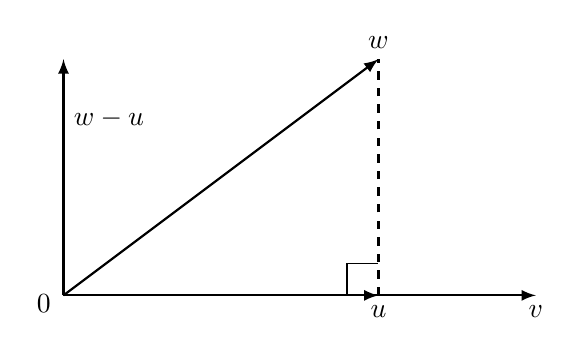
\begin{tikzpicture}
  \coordinate (v1) at (0,0);
  \coordinate (v2) at (4,3);
  \coordinate (v3) at (6,0);
  \coordinate (v4) at (4,0);
  \coordinate (v5) at (0,3);
  \path[draw] (3.6,0) -- (3.6,0.4) -- (4,0.4);
  \node (v0) at (-0.25,-0.1) {$\vecnot{0}$};
  \draw[-latex,thick] (v1) -- node[at end,above] {$\vecnot{w}$} (v2);
  \draw[-latex,thick] (v1) -- node[at end,below] {$\vecnot{v}$} (v3);
  \draw[-latex,thick] (v1) -- node[at end, below] {$\vecnot{u}$} (v4);
  \draw[thick,dashed] (v4) --  (v2);
  \draw[-latex,thick] (v1) -- node[right,near end] {$\vecnot{w}-\vecnot{u}$} (v5);
\end{tikzpicture}
\caption{\label{fig:vector_projection}The projection of $\vecnot{w}$ onto $\vecnot{v}$ is given by $\vecnot{u}$ and $\vecnot{w}-\vecnot{u}$ is orthogonal to $\vecnot{v}$.}
\end{figure}

\begin{definition}
Let $\vecnot{w},\vecnot{v}$ be vectors in an inner-product space $V$ with inner product $\langle \cdot | \cdot \rangle$.
As shown in Figure~\ref{fig:vector_projection}, the \defn{inner-product space}{projection} of $\vecnot{w}$ onto $\vecnot{v}$ is defined to be
\begin{equation*}
\vecnot{u} = \frac{\left\langle \vecnot{w} | \vecnot{v} \right\rangle}{\|\vecnot{v}\|^2} \vecnot{v}
\end{equation*}
\end{definition}

\begin{lemma} \label{lem:proj_loss}
Let $\vecnot{u}$ be the projection of $\vecnot{w}$ onto $\vecnot{v}$.
Then, $\langle \vecnot{w}-\vecnot{u} | \vecnot{u} \rangle = 0$ and
\[ \|\vecnot{w}-\vecnot{u}\|^2 =  \|\vecnot{w}\|^2 - \| \vecnot{u} \|^2 = \|\vecnot{w}\|^2 - \frac{|\langle \vecnot{w} | \vecnot{v} \rangle|^2}{\|\vecnot{v}\|^2}. \]
\end{lemma}
\begin{proof}
First, we observe that
\[ \langle \vecnot{w} - \vecnot{u} | \vecnot{v} \rangle = \langle \vecnot{w} | \vecnot{v} \rangle - \langle \vecnot{u} | \vecnot{v} \rangle = \langle \vecnot{w} | \vecnot{v} \rangle - \frac{\left\langle \vecnot{w} | \vecnot{v} \right\rangle}{\|\vecnot{v}\|^2} \langle \vecnot{v} | \vecnot{v} \rangle = 0. \]
Since $\vecnot{u} = s \vecnot{v}$ for some scalar $s$, it follows that $\langle \vecnot{w}-\vecnot{u} | \vecnot{u} \rangle = \overline{s} \langle \vecnot{w}-\vecnot{u} | \vecnot{v} \rangle =  0$.
Using $\langle \vecnot{w}-\vecnot{u} | \vecnot{u} \rangle = 0$, we can write
\begin{align*}
\|\vecnot{w}\|^2 &= \|(\vecnot{w}-\vecnot{u})+\vecnot{u}\|^2
= \langle (\vecnot{w}-\vecnot{u})+\vecnot{u}|(\vecnot{w}-\vecnot{u})+\vecnot{u}\rangle \\
&= \|\vecnot{w}-\vecnot{u}\|^2 + 2 \Real \langle \vecnot{w}-\vecnot{u} | \vecnot{u} \rangle + \|\vecnot{u}\|^2
= \|\vecnot{w}-\vecnot{u}\|^2 + \|\vecnot{u}\|^2.
\end{align*}
The proof is completed by noting that $\|\vecnot{u}\|^2 = |\langle \vecnot{w} | \vecnot{v} \rangle|^2 / \|\vecnot{v}\|^2$.
\end{proof}

\begin{theorem}
If $V$ is an inner-product space and $\| \cdot \|$ is its associated induced norm, then for any $\vecnot{v}, \vecnot{w} \in V$ and any scalar $s$
\begin{enumerate}
\item $\left\| s \vecnot{v} \right\| = |s| \left\| \vecnot{v} \right\|$
\item $\left\| \vecnot{v} \right\| > 0$ for $\vecnot{v} \neq \vecnot{0}$
\item $\left| \left\langle \vecnot{v} | \vecnot{w} \right\rangle \right| \leq \left\| \vecnot{v} \right\| \left\| \vecnot{w} \right\|$ with equality iff $\vecnot{v} = \vecnot{0}$, $\vecnot{w}=\vecnot{0}$, or $\vecnot{v} = s \vecnot{w}$
\item $\left\| \vecnot{v} + \vecnot{w} \right\| \leq \left\| \vecnot{v} \right\| + \left\| \vecnot{w} \right\|$ with equality iff $\vecnot{v} = \vecnot{0}$, $\vecnot{w}=\vecnot{0}$, or $\vecnot{v} = s \vecnot{w}$.
\end{enumerate}
\end{theorem}
\begin{proof}
The first two items follow immediately from the definitions involved.
The third inequality, $\left| \left\langle \vecnot{v} | \vecnot{w} \right\rangle \right| \leq \left\| \vecnot{v} \right\| \left\| \vecnot{w} \right\|$, is called the \defn{inner-product space}{Cauchy-Schwarz inequality}.
When $\vecnot{v} = \vecnot{0}$, then clearly $\left| \left\langle \vecnot{v} | \vecnot{w} \right\rangle \right| = \left\| \vecnot{v} \right\| \left\| \vecnot{w} \right\| =0$.
Assume $\vecnot{v} \neq \vecnot{0}$ and let
\begin{equation*}
\vecnot{u} = \frac{ \left\langle \vecnot{w} | \vecnot{v} \right\rangle}{ \left\| \vecnot{v} \right\|^2 } \vecnot{v}
\end{equation*}
be the projection $\vecnot{w}$ onto $\vecnot{v}$.
By Lemma~\ref{lem:proj_loss},
we have
%$\left\langle \vecnot{w} - \vecnot{u} | \vecnot{v} \right\rangle = 0$ and
\begin{align*}
0 &\leq \left\| \vecnot{w} - \vecnot{u} \right\|^2
%= \left\langle \vecnot{u} \,\middle|\, \vecnot{w} - \frac{ \left\langle \vecnot{w} | \vecnot{v} \right\rangle}{ \left\| \vecnot{v} \right\|^2 } \vecnot{v} \right\rangle = \left\langle \vecnot{u} \,\middle|\, \vecnot{w} \right\rangle
%= \left\langle \vecnot{w} - \frac{ \left\langle \vecnot{w} | \vecnot{v} \right\rangle}{ \left\| \vecnot{v} \right\|^2 } \vecnot{v} \,\middle|\, \vecnot{w}
% \right\rangle \\
%&= \left\langle \vecnot{w} | \vecnot{w} \right\rangle
%- \frac{ \left\langle \vecnot{w} | \vecnot{v} \right\rangle
%\left\langle \vecnot{v} | \vecnot{w} \right\rangle}
%{ \left\| \vecnot{v} \right\|^2 }
= \left\| \vecnot{w} \right\|^2
- \frac{ \left| \left\langle \vecnot{w} | \vecnot{v} \right\rangle \right|^2 }
{ \left\| \vecnot{v} \right\|^2 } ,
\end{align*}
where equality holds iff $\vecnot{w}-\vecnot{u}=\vecnot{0}$, or equivalently iff $\vecnot{w}=\vecnot{0}$ or $\vecnot{v} = s \vecnot{w}$.
Hence, we find that
$\left| \left\langle \vecnot{v} | \vecnot{w} \right\rangle \right|^2 = \left| \left\langle \vecnot{w} | \vecnot{v} \right\rangle \right|^2 \leq \left\| \vecnot{v} \right\|^2 \left\| \vecnot{w} \right\|^2$.
%with equality iff $\vecnot{v}=\vecnot{0}$, $\vecnot{w}=\vecnot{0}$, or $\vecnot{v} = s \vecnot{w}$.
%Note that the $\vecnot{v}=\vecnot{0}$ case is checked separately because it is assumed above that $\vecnot{v}\neq \vecnot{0}$.
Using this result, it follows that
\begin{equation*}
\begin{split}
\left\| \vecnot{v} + \vecnot{w} \right\|^2
&= \left\| \vecnot{v} \right\|^2 + \left\langle \vecnot{v} | \vecnot{w} \right\rangle + \left\langle \vecnot{w} | \vecnot{v} \right\rangle + \left\| \vecnot{w} \right\|^2 \\
&= \left\| \vecnot{v} \right\|^2 + 2 \Real \left\langle \vecnot{v} | \vecnot{w} \right\rangle + \left\| \vecnot{w} \right\|^2 \\
&\leq \left\| \vecnot{v} \right\|^2 + 2 \left\| \vecnot{v} \right\| \left\| \vecnot{w} \right\| + \left\| \vecnot{w} \right\|^2 ,
\end{split}
\end{equation*}
with equality iff Cauchy-Schwarz holds with equality.
Thus, $\left\| \vecnot{v} + \vecnot{w} \right\| \leq \left\| \vecnot{v} \right\| + \left\| \vecnot{w} \right\|$ with equality iff $\vecnot{v} = \vecnot{0}$, $\vecnot{w}=\vecnot{0}$, or $\vecnot{v} = s \vecnot{w}$ (i.e., $\vecnot{v}$ and $\vecnot{w}$ are linearly dependent).
\end{proof}

%Its proof shows that if $\vecnot{v}$ is non-zero, then $\left| \left\langle \vecnot{v} | \vecnot{w} \right\rangle \right| < \left\| \vecnot{v} \right\| \left\| \vecnot{w} \right\|$ unless
%\begin{equation*}
%\vecnot{w} = \frac{ \left\langle \vecnot{w} | \vecnot{v} \right\rangle }
%{ \left\| \vecnot{v} \right\| } \vecnot{v} .
%\end{equation*}
%That is, equality holds if and only if $\vecnot{v}$ and $\vecnot{w}$ are linearly dependent.

\begin{theorem}
\label{theorem:InnerProductContinuous}
Consider the vector space $\RealNumbers^n$ with the standard inner product. % of Example~\ref{example:StandardInnerProduct}.
Then, the function $f \colon V \rightarrow F$ defined by $f \left( \vecnot{w} \right) = \left\langle \vecnot{w} | \vecnot{v} \right\rangle$ is continuous.
\end{theorem}
\begin{proof}
Let $\vecnot{w}_1, \vecnot{w}_2, \ldots$ be a sequence in $V$ converging to $\vecnot{w}$.
Then,
\begin{equation*}
\left| \left\langle \vecnot{w}_n | \vecnot{v} \right\rangle
- \left\langle \vecnot{w} | \vecnot{v} \right\rangle \right|
= \left| \left\langle \vecnot{w}_n - \vecnot{w} | \vecnot{v} \right\rangle \right|
\leq \left\| \vecnot{w}_n - \vecnot{w} \right\| \left\| \vecnot{v} \right\|.
\end{equation*}
Since $\left\| \vecnot{w}_n - \vecnot{w} \right\| \rightarrow 0$, the convergence of $\left\langle \vecnot{w}_n, \vecnot{v} \right\rangle$ is established.
\end{proof}


\section{Sets of Orthogonal Vectors}

\begin{definition}
Let $V$ be an inner-product space and $U,W$ be subspaces.
Then, the subspace $U$ is an \defn{inner-product space}{orthogonal} to the subspace $W$ (denoted $U \bot W$) if $\vecnot{u} \bot \vecnot{w}$ for all $\vecnot{u}\in U$ and $\vecnot{w}\in W$.
\end{definition}

\begin{definition}
A collection $W$ of vectors in $V$ is an \defn{inner-product space}{orthogonal set} if all pairs of distinct vectors in $W$ are orthogonal.
\end{definition}

\begin{example}
The standard basis of $\RealNumbers^n$ is an orthonormal set with respect to the standard inner product.
\end{example}

\begin{example}
Let $V$ be the vector space (over $\ComplexNumbers$) of continuous complex-valued functions on the interval $0 \leq x \leq 1$ with the inner product
\begin{equation*}
\left\langle f | g \right\rangle = \int_0^1 f(x) \overline{g(x)} dx.
\end{equation*}
Let $f_n(x) = \sqrt{2} \cos 2 \pi n x$ and $g_n (x) = \sqrt{2} \sin 2 \pi n x$.
Then $\{ 1, f_1, g_1, f_2, g_2, \ldots \}$ is a countably infinite orthonormal set that is a Schauder basis for this vector space.
\end{example}

\begin{theorem}
An orthogonal set of non-zero vectors is linearly independent.
\end{theorem}
\begin{proof}
Let $W$ be an orthogonal set of non-zero vectors in a given inner-product space $V$.
Suppose $\vecnot{w}_1, \ldots, \vecnot{w}_n$ are distinct vectors in $W$ and consider
\begin{equation*}
\vecnot{v} = s_1 \vecnot{w}_1 + \cdots + s_n \vecnot{w}_n.
\end{equation*}
The inner product $\left\langle \vecnot{v} | \vecnot{w}_i \right\rangle$ is given by
\begin{equation*}
\begin{split}
\left\langle \vecnot{v} | \vecnot{w}_i \right\rangle
&= \left\langle \sum_j s_j \vecnot{w}_j | \vecnot{w}_i \right\rangle
= \sum_j s_j \left\langle \vecnot{w}_j | \vecnot{w}_i \right\rangle
= s_i \left\langle \vecnot{w}_i | \vecnot{w}_i \right\rangle .
\end{split}
\end{equation*}
Since $\left\langle \vecnot{w}_i | \vecnot{w}_i \right\rangle \neq 0$, it follows that
\begin{equation*}
s_i = \frac{ \left\langle \vecnot{v} | \vecnot{w}_i \right\rangle }
{ \left\| \vecnot{w}_i \right\|^2 }
\quad 1 \leq i \leq n.
\end{equation*}
In particular, if $\vecnot{v} = 0$ then $s_j = 0$ for $1 \leq j \leq n$ and the vectors in $W$ are linearly independent.
\end{proof}

\begin{corollary}
If $\vecnot{v} \in V$ is a linear combination of an orthogonal sequence of distinct, non-zero vectors $\vecnot{w}_1, \ldots, \vecnot{w}_n$, then $\vecnot{v}$ satisfies the identity
\begin{equation*}
\vecnot{v} = \sum_{i = 1}^n \frac{ \left\langle \vecnot{v} | \vecnot{w}_i \right\rangle } { \left\| \vecnot{w}_i \right\|^2 } \vecnot{w}_i,
\end{equation*}
and equals the sum of the projections of $\vecnot{v}$ onto $\vecnot{w}_1, \ldots, \vecnot{w}_n$.
\end{corollary}

\begin{theorem}
Let $V$ be an inner-product space and assume $\vecnot{v}_1, \ldots, \vecnot{v}_n$ are linearly independent vectors in $V$.
Then it is possible to construct an orthogonal sequence of vectors $\vecnot{w}_1, \ldots, \vecnot{w}_n \in V$ such that for each $k = 1, \ldots, n$ the set
\begin{equation*}
\left\{ \vecnot{w}_1, \ldots, \vecnot{w}_k \right\}
\end{equation*}
is a basis for the subspace spanned by $\vecnot{v}_1, \ldots, \vecnot{v}_k$.
\end{theorem}
\begin{proof}
First, let $\vecnot{w}_1 = \vecnot{v}_1$.
The remaining vectors are defined inductively as part during the proof.
Suppose the vectors
\begin{equation*}
\vecnot{w}_1, \ldots, \vecnot{w}_m \quad (1 \leq m < n)
\end{equation*}
have been chosen so that for every $k$
\begin{equation*}
\left\{ \vecnot{w}_1, \ldots, \vecnot{w}_k \right\} \quad 1 \leq k \leq m
\end{equation*}
is an orthogonal basis for the subspace spanned by $\vecnot{v}_1, \ldots, \vecnot{v}_k$.
Let
\begin{equation*}
\vecnot{w}_{m+1} = \vecnot{v}_{m+1} - \sum_{i=1}^m \frac{ \left\langle \vecnot{v}_{m+1} | \vecnot{w}_i \right\rangle } { \left\| \vecnot{w}_i \right\|^2 } \vecnot{w}_i.
\end{equation*}
Then $\vecnot{w}_{m+1} \neq 0$, for otherwise $\vecnot{v}_{m+1}$ is a linear combination of $\vecnot{w}_1, \ldots, \vecnot{w}_m$ and hence a linear combination of $\vecnot{v}_1, \ldots, \vecnot{v}_m$.
For $j \in \{1, \ldots, m\}$, we also have
\begin{equation*}
\begin{split}
\left\langle \vecnot{w}_{m+1} | \vecnot{w}_j \right\rangle
&= \left\langle \vecnot{v}_{m+1} | \vecnot{w}_j \right\rangle
- \sum_{i=1}^m \frac{ \left\langle \vecnot{v}_{m+1} | \vecnot{w}_i \right\rangle } { \left\| \vecnot{w}_i \right\|^2 }
\left\langle \vecnot{w}_i | \vecnot{w}_j \right\rangle \\
&= \left\langle \vecnot{v}_{m+1} | \vecnot{w}_j \right\rangle
- \frac{ \left\langle \vecnot{v}_{m+1} | \vecnot{w}_j \right\rangle } { \left\| \vecnot{w}_j \right\|^2 }
\left\langle \vecnot{w}_j | \vecnot{w}_j \right\rangle \\
&= 0.
\end{split}
\end{equation*}
Clearly, $\{ \vecnot{w}_1, \ldots, \vecnot{w}_{m+1} \}$ is an orthogonal set consisting of $m+1$ non-zero vectors in the subspace spanned by $\vecnot{v}_1, \ldots, \vecnot{v}_{m+1}$.
Since the dimension of the latter subspace is $m+1$, this set is a basis for the subspace.
\end{proof}

The inductive construction of the vectors $\vecnot{w}_1, \ldots, \vecnot{w}_n$ is known as the \defn{inner-product space}{Gram-Schmidt orthogonalization} process.

\begin{corollary}
\label{cor:orthonormal_basis}
Every finite-dimensional inner-product space has a basis of orthonormal vectors.
\end{corollary}
\begin{proof}
Let $V$ be a finite-dimensional inner-product space.
Suppose that $\vecnot{v}_1, \ldots, \vecnot{v}_n$ is a basis for $V$.
Apply the Gram-Schmidt process to obtain a basis of orthogonal vectors $\vecnot{w}_1, \ldots, \vecnot{w}_n$.
Then, a basis of orthonormal vectors is given by
\begin{equation*}
\vecnot{u}_1 = \frac{ \vecnot{w}_1 }{ \left\| \vecnot{w}_1 \right\| }, \ldots,
\vecnot{u}_n = \frac{ \vecnot{w}_n }{ \left\| \vecnot{w}_n \right\| }.
\end{equation*}
\end{proof}

\begin{example}
Consider the vectors
\begin{align*}
\vecnot{v}_1 &= (2,2,1) \\
\vecnot{v}_2 &= (3,6,0) \\
\vecnot{v}_3 &= (6,3,9)
\end{align*}
in $\RealNumbers^3$ equipped with the standard inner product.
Apply the Gram-Schmidt process to $\vecnot{v}_1, \vecnot{v}_2, \vecnot{v}_3$ to obtain an orthogonal basis.

Applying the Gram-Schmidt process to $\vecnot{v}_1, \vecnot{v}_2, \vecnot{v}_3$, we get
\begin{align*}
\vecnot{w}_1 &= (2,2,1) \\
\vecnot{w}_2 &= (3,6,0)
- \frac{ \left\langle (3,6,0) | (2,2,1) \right\rangle }{ 9 } (2,2,1) \\
&= (3,6,0) - 2 (2,2,1) = (-1,2,-2) \\
\vecnot{w}_3 &= (6,3,9)
- \frac{ \left\langle (6,3,9) | (2,2,1) \right\rangle }{ 9 } (2,2,1)
- \frac{ \left\langle (6,3,9) | (-1,2,-2) \right\rangle }{ 9 } (-1,2,-2) \\
&= (6,3,9) - 3 (2,2,1) + 2 (-1,2,-2) = (-2,1,2) .
\end{align*}
It is easily verified that $\vecnot{w}_1, \vecnot{w}_2, \vecnot{w}_3$ is an orthogonal set of vectors.
\end{example}

\begin{definition}
Let $V$ be an inner-product space and $W$ be any set of vectors in $V$.
The \defn{inner-product space}{orthogonal complement} of $W$ denoted by $W^{\bot}$ is the set of all vectors in $V$ that are orthogonal to every vector in $W$ or
\begin{equation*}
W^{\bot} = \left\{ \vecnot{v} \in V \big| \langle \vecnot{v} | \vecnot{w} \rangle = 0 \; \forall \; \vecnot{w}\in W \right\}. 
\end{equation*}
\end{definition}

\begin{problem} \label{problem:WbotSubspace}
Let $W$ be any subset of vector space $V$.
Show that $W^{\bot}$ is a closed subspace of $V$ and that any vector in the subspace spanned by $W$ is orthogonal to any vector in $W^{\bot}$.
\end{problem}
\noindent
\textbf{S~\ref{problem:WbotSubspace}}.
Let $\vecnot{m}_1, \vecnot{m}_2 \in W^{\bot}$ and $s \in F$.
For any vector $\vecnot{w} \in W$, we have
\begin{equation*}
\left\langle \vecnot{m}_1 | \vecnot{w} \right\rangle
= \left\langle \vecnot{m}_2 | \vecnot{w} \right\rangle
= 0.
\end{equation*}
This implies
\begin{equation*}
\left\langle s \vecnot{m}_1 + \vecnot{m}_2 | \vecnot{w} \right\rangle
= s \left\langle \vecnot{m}_1 | \vecnot{w} \right\rangle
+ \left\langle \vecnot{m}_2 | \vecnot{w} \right\rangle
= 0.
\end{equation*}
That is, $s \vecnot{m}_1 + \vecnot{m}_2 \in W^{\bot}$.
Hence, $W^{\bot}$ is a subspace of $V$.

To see that $W^{\bot}$ is closed, we let $\vecnot{m}$ be any point in the closure of $W^{\bot}$ and $\vecnot{m}_1,\vecnot{m}_2,\ldots \in W^{\bot}$ be a sequence that converges to $\vecnot{m}$.
The continuity of the inner product, from Theorem~\ref{theorem:InnerProductContinuous}, implies that, for all $\vecnot{w}\in W$,
\[ \left\langle \vecnot{m} | \vecnot{w} \right\rangle =  \left\langle \lim_{n\rightarrow\infty} \vecnot{m}_n | \vecnot{w}  \right\rangle  =  \lim_{n\rightarrow\infty}  \left\langle \vecnot{m}_n | \vecnot{w}  \right\rangle = 0. \]
Therefore, $\vecnot{m} \in W^{\bot}$ and the orthogonal complement contains all of its limit points.

Notice also that any vector $\vecnot{w}$ in the subspace spanned by $W$ can be written as $\vecnot{w} = \sum_{i} s_i \vecnot{w}_i$ with $\vecnot{w}_i \in W$ and $s_i \in F$.
Therefore, the inner product of $\vecnot{w}$ with any $\vecnot{w}' \in W^{\bot}$ is given by
\begin{equation*}
\left\langle \vecnot{w} | \vecnot{w}' \right\rangle
= \left\langle \sum_{i} s_i \vecnot{w}_i \Big| \vecnot{w}' \right\rangle \\
= \sum_{i} s_i \left\langle \vecnot{w}_i | \vecnot{w}' \right\rangle \\
= 0.
\end{equation*}
It follows that the subspace spanned by $W$ is orthogonal to the subspace $W^{\bot}$.

\begin{definition}
A complex matrix $U\in \ComplexNumbers^{n\times n}$ is called \defn{inner-product space}{unitary} if $U^H U = I$.
Similarly, a real matrix $Q\in \RealNumbers^{n\times n}$ is called \defn{inner-product space}{orthogonal} if $Q^T Q = I$.
\end{definition}

\begin{theorem}
Let $V = \ComplexNumbers^n$ be the standard inner product space and let  $U\in \ComplexNumbers^{n\times n}$ define a linear operator on $V$.
Then, the following conditions are equivalent:
\begin{enumerate}
\item[(i)] The columns of $U$ form an orthonormal basis (i.e.,  $U^H U = I$),
\item[(ii)] the rows of $U$ form an orthonormal basis (i.e.,  $U U^H = I$),
\item[(iii)] $U$ preserves inner products (i.e., $\langle U \vecnot{v} | U \vecnot{w} \rangle = \langle \vecnot{v} | \vecnot{w} \rangle$ for all $\vecnot{u},\vecnot{v}\in V$), and
\item[(iv)] $U$ is an isometry (i.e., $\| U \vecnot{v} \| = \| \vecnot{v}\|$ for all $\vecnot{v} \in V$).
\end{enumerate}
\end{theorem}
\begin{proof}
If {\it(i)} holds, then $U$ is invertible because its columns are linearly independent.
Thus, $U^H U = I$ implies $U^H = U^{-1}$ and {\it(ii)} follows.
Likewise, {\it(iii)} holds because $\langle U \vecnot{v} | U \vecnot{w} \rangle = \vecnot{w}^H U^H U \vecnot{v} = \vecnot{w}^H \vecnot{v} = \langle \vecnot{v} | \vecnot{w} \rangle$ for all $\vecnot{u},\vecnot{v}\in V$.
Choosing $\vecnot{w}=\vecnot{v}$ gives {\it(iv)}.
Lastly, if $\| U \vecnot{v} \| = \| \vecnot{v}\|$ for all $\vecnot{v} \in V$, then
$\vecnot{v}^H (U^H U - I) \vecnot{v} = \| U \vecnot{v} \|^2 - \| \vecnot{v} \|^2 = 0$ for all $\vecnot{v} \in V$.
Since $U^H U - I$ is Hermitian, it must have a complete set of eigenvectors but all eigenvalues must be 0.  Thus, $U^H U - I = 0$.
\end{proof}

\subsection{Hilbert Spaces}

\begin{definition}
A complete inner-product space is called a \defn{inner-product space}{Hilbert space}.
\end{definition}

\begin{definition}
Recall that a subset $\left\{ \vecnot{v}_{\alpha} | \alpha \in A \right\}$ of a Hilbert space $V$ is said to be orthonormal if $\left\| \vecnot{v}_{\alpha} \right\| = 1$ for every $\alpha \in A$ and $\left\langle \vecnot{v}_{\alpha} | \vecnot{v}_{\beta} \right\rangle = 0$ for all $\alpha \neq \beta$.
If the subspace spanned by the family $\left\{ \vecnot{v}_{\alpha} | \alpha \in A \right\}$ is dense in $V$, we call this set an \defn{inner-product space}{orthonormal basis}.
\end{definition}

Note that, according to this definition, an orthonormal basis for a Hilbert space $V$ is not necessarily a Hamel basis for $V$.
However, it can be shown that any orthogonal basis is a subset of a Hamel basis.
In practice it is the orthonormal basis, not the Hamel basis itself, which is of most use.
None of these issues arise in finite-dimensional spaces, where an orthogonal basis is always a Hamel basis.

Let $\mathcal{B} = \left\{ \vecnot{v}_{\alpha} | \alpha \in A \right\}$ be an orthonormal basis for Hilbert space $V$.
Then, each element $\vecnot{v} \in V$ has a unique representation as
\begin{equation*}
\vecnot{v} = \sum_{\alpha \in A} s_{\alpha} \vecnot{v}_{\alpha}.
\end{equation*}
Using orthogonality to compute $\left\langle \vecnot{v} | \vecnot{v} \right\rangle$, one gets the \defn{inner-product space}{Parseval identity}
\begin{equation*}
\left\| \vecnot{v} \right\|^2 = \sum_{\alpha \in A} | s_{\alpha} |^2.
\end{equation*}
Since $\| \vecnot{v} \|^2 < \infty$ for all $\vecnot{v} \in V$, the RHS also exists and is finite for all $\vecnot{v} \in V$.

\begin{theorem}
Every orthogonal set in a Hilbert space $V$ can be enlarged to an orthonormal basis for $V$.
\end{theorem}
\begin{proof}
Let $X$ be the set of orthonormal subsets of $V$.
Furthermore, for $x, y \in X$ consider the strict partial order defined by proper inclusion.
If $x = \left\{ \vecnot{v}_{\alpha} | \alpha \in A_0 \right\}$ is an element of $X$, then by the Hausdorff maximal principle there exists a maximal simply ordered subset $Z$ of $X$ containing $x$.
This shows the existence of a maximal orthonormal set $\left\{ \vecnot{v}_{\alpha} | \alpha \in A \right\}$, where $A_0 \subset A$.

Let $W$ be the closed subspace of $V$ generated by $\left\{ \vecnot{v}_{\alpha} | \alpha \in A \right\}$.
If $W \neq V$, there is a unit vector $\vecnot{u} \in W^{\bot}$, contradicting the maximality of the system $\left\{ \vecnot{v}_{\alpha} | \alpha \in A \right\}$.
Thus, $W = V$ and we have an orthonormal basis.
\end{proof}

\begin{theorem} \label{theorem:SeparableHilbertSpace}
A Hilbert space $V$ has a countable orthonormal basis if and only if $V$ is separable.
\end{theorem}
\begin{proof}[Sketch of proof]
If $V$ is separable, then it contains a countable dense subset.
Using the well-ordering theorem, this subset can be ordered into a sequence $\vecnot{v}_1 , \vecnot{v}_2 , \ldots$ such that, for every vector $\vecnot{v}\in V$ and any $\epsilon>0$, there exists an $n$ such that $\left\| \vecnot{v} - \vecnot{v}_n \right\| < \epsilon$.
A countable orthonormal basis is generated by applying Gram-Schmidt orthogonalization to this ordered sequence of vectors.
Conversely, if $V$ has a countable orthonormal basis, then linear combinations with rational coefficients can be used to construct a countable dense subset.
\end{proof}

\begin{lemma} \label{lem:hilbert_sum_convergence}
Let $V$ be a Hilbert space and $\vecnot{v_1},\vecnot{v}_2,\ldots$ be a countable orthogonal set.
Then, $\vecnot{v} = \sum_{i=1}^\infty \vecnot{v}_i$ exists if and only $\sum_{i=1}^\infty \|\vecnot{v}_i\|^2 = M < \infty$.
\end{lemma}
\begin{proof}
For $\vecnot{u}_n = \sum_{i=1}^n \vecnot{v}_i$ and $w_n = \sum_{i=1}^n \|\vecnot{v}_i\|^2$, orthogonality implies that
\[\|\vecnot{u}_m - \vecnot{u}_n\|^2 = \left\| \sum_{i=n+1}^m \vecnot{v}_i \right\|^2 = \sum_{i=n+1}^m \|\vecnot{v}_i \|^2 = | w_m - w_n|. \]
Thus, the sequence $\vecnot{u}_n$ is Cauchy in $V$ if and only if $w_n$ is Cauchy in $\RealNumbers$.
\end{proof}


\section{Linear Functionals}

\begin{definition}
Let $V$ be a vector space over a field $F$.
A linear transformation $f$ from $V$ into the scalar field $F$ is called a \defn{vector space}{linear functional} on $V$.
\end{definition}
That is, $f$ is a functional on $V$ such that
\begin{equation*}
f \left( s \vecnot{v}_1 + \vecnot{v}_2 \right)
= s f \left( \vecnot{v}_1 \right) + f \left( \vecnot{v}_2 \right)
\end{equation*}
for all $\vecnot{v}_1, \vecnot{v}_2 \in V$ and $s \in F$.

\begin{example}
Let $F$ be a field and let $s_1, \ldots, s_n$ be scalars in $F$.
Then the functional $f$ on $F^n$ defined by
\begin{equation*}
f(v_1, \ldots, v_n) = s_1 v_1 + \cdots + s_n v_n
\end{equation*}
is a linear functional.
It is the linear functional which is represented by the matrix
\begin{equation*}
\begin{bmatrix} s_1 & s_2 & \cdots & s_n \end{bmatrix}
\end{equation*}
relative to the standard ordered basis for $F^n$.
Every linear functional on $F^n$ is of this form, for some scalars $s_1, \ldots, s_n$.
\end{example}

\begin{definition}
Let $n$ be a positive integer and $F$ a field.
If $A$ is an $n \times n$ matrix with entries in $F$, the \defn{matrix}{trace} of $A$ is the scalar
\begin{equation*}
\Trace(A) = A_{11} + A_{22} + \cdots + A_{nn}.
\end{equation*}
\end{definition}

\begin{example}
The trace function is a linear functional on the matrix space $F^{n \times n}$ since
\begin{equation*}
\begin{split}
\Trace ( sA + B) &= \sum_{i=1}^n (s A_{ii} + B_{ii}) \\
&= s \sum_{i=1}^n A_{ii} + \sum_{i=1}^n  B_{ii} \\
&= s \; \Trace(A) + \Trace(B) .
\end{split}
\end{equation*}
\end{example}

\begin{example}
Let $[a, b]$ be a closed interval on the real line and let $C([a,b])$ be the space of continuous real-valued functions on $[a,b]$.
Then
\begin{equation*}
L(g) = \int_a^b g(t) dt
\end{equation*}
defines a linear functional $L$ on $C([a,b])$.
\end{example}

\begin{theorem}[Riesz] \label{theorem:riesz_finite}
Let $V$ be a finite-dimensional Hilbert space and $f$ be a linear functional on $V$.
Then, there exists a unique vector $\vecnot{v} \in V$ such that $f \left( \vecnot{w} \right) = \left\langle \vecnot{w} | \vecnot{v} \right\rangle$ for all $\vecnot{w} \in V$.
\end{theorem}

\begin{proof}
%Now, we can take a closer look at the proof of this theorem for the finite dimensional case.
If we choose an orthonormal basis $\mathcal{B} = \vecnot{v}_1, \ldots, \vecnot{v}_n$ for $V$, then the inner product of $\vecnot{w} = t_1 \vecnot{v}_1 + \cdots + t_n \vecnot{v}_n$ and $\vecnot{v} = s_1 \vecnot{v}_1 + \cdots + s_n \vecnot{v}_n$ will be
\begin{equation*}
\left\langle \vecnot{w} | \vecnot{v} \right\rangle = t_1 \bar{s}_1 + \cdots + t_n \bar{s}_n .
\end{equation*}
If $f$ is a linear functional on $V$, then $f$ has the form
\begin{equation*}
f \left(\vecnot{w}\right) = f(t_1 \vecnot{v}_1 + \cdots + t_n \vecnot{v}_n) = t_1 f \left( \vecnot{v}_1 \right) + \cdots + t_n f \left( \vecnot{v}_n \right).
\end{equation*}
Thus, we can choose $\bar{s}_j = f \left( \vecnot{v}_j \right)$ to get $ \left\langle \vecnot{w} | \vecnot{v} \right\rangle = f \left( \vecnot{w} \right)$ and this gives
\begin{equation*}
\vecnot{v} = \overline{ f \left( \vecnot{v}_1 \right) } \vecnot{v}_1 + \cdots + \overline{ f \left( \vecnot{v}_n \right) } \vecnot{v}_n .
\end{equation*}

Let $\vecnot{v}'$ be any vector that satisfies $f \left( \vecnot{w} \right) = \left\langle \vecnot{w} | \vecnot{v}' \right\rangle$ for all $\vecnot{w}\in V$.
Then, we see that $\left\langle \vecnot{w} | \vecnot{v} - \vecnot{v}' \right\rangle = 0$
for all $\vecnot{w}\in V$.
This implies that $\vecnot{v}-\vecnot{v}' = \vecnot{0}$.

\iffalse

Thus, the vector $\vecnot{v}$ is unique.
 for some fixed scalars $c_1, \ldots, c_n$ determined by the basis.
Clearly, $f \left( \vecnot{v}_j \right) = c_j$, which implies that $\bar{s}_j = f \left( \vecnot{v}_j \right)$.
That is, the vector $\vecnot{v}$ such that $f \left( \vecnot{w} \right) = \left\langle \vecnot{w} | \vecnot{v} \right\rangle$ is

Note that the vector $\vecnot{v}$ lies in the orthogonal complement of the nullspace of $f$.
Let $W$ be the nullspace of $f$, then $V = W \oplus W^{\bot}$, and $f$ is completely determined by its value on $W^{\bot}$.
In fact, if $P$ gives the orthogonal projection of $V$ on $W^{\bot}$, then
\begin{equation*}
f \left( \vecnot{u} \right) = f \left( P \vecnot{u} \right)
\end{equation*}
for all $\vecnot{u} \in V$.
Suppose that $f \neq 0$, then $f$ is of rank one and $\dim \left( W^{\bot} \right) = 1$.
If $\vecnot{v}$ is any non-zero vector in $W^{\bot}$, it follows that
\begin{equation*}
P \vecnot{u} = \frac{ \left\langle \vecnot{u} | \vecnot{v} \right\rangle }{ \left\| \vecnot{v} \right\|^2 } \vecnot{v}
\end{equation*}
for all $\vecnot{u} \in V$.
Thus,
\begin{equation*}
f \left( \vecnot{u} \right) = \left\langle \vecnot{u} | \vecnot{v} \right\rangle
\frac{f \left( \vecnot{v} \right) }{ \left\| \vecnot{v} \right\|^2 }
\end{equation*}
for all $\vecnot{u} \in V$.
\fi

\end{proof}
